%\documentclass[review]{elsarticle}
\documentclass{elsarticle}


\usepackage{lineno,hyperref}
\modulolinenumbers[5]

\journal{Computers \& Fluids}

%%%%%%%%%%%%%%%%%%%%%%%
%% Elsevier bibliography styles
%%%%%%%%%%%%%%%%%%%%%%%
%% To change the style, put a % in front of the second line of the current style and
%% remove the % from the second line of the style you would like to use.
%%%%%%%%%%%%%%%%%%%%%%%

%% Numbered
%\bibliographystyle{model1-num-names}

%% Numbered without titles
%\bibliographystyle{model1a-num-names}

%% Harvard
%\bibliographystyle{model2-names.bst}\biboptions{authoryear}

%% Vancouver numbered
%\usepackage{numcompress}\bibliographystyle{model3-num-names}

%% Vancouver name/year
%\usepackage{numcompress}\bibliographystyle{model4-names}\biboptions{authoryear}

%% APA style
%\bibliographystyle{model5-names}\biboptions{authoryear}

%% AMA style
%\usepackage{numcompress}\bibliographystyle{model6-num-names}

%% `Elsevier LaTeX' style
\bibliographystyle{elsarticle-num}
%%%%%%%%%%%%%%%%%%%%%%%

\graphicspath{{./}{./FIGURES/}}
\usepackage{listings}


\newcommand{\be}[1]{ \begin{equation} \label{#1}}
\newcommand{\ee}{\end{equation}}

\begin{document}

\begin{frontmatter}

\title{Popularizing linear and nonlinear approaches to global flow instabilities : 
A review and a simple implementation for the wake of a cylinder (and of a sphere ?)}%\tnoteref{mytitlenote}}

%\tnotetext[mytitlenote]{Fully documented templates are available in the elsarticle package on \href{http://www.ctan.org/tex-archive/macros/latex/contrib/elsarticle}{CTAN}.}

%% Group authors per affiliation:
\author{D. Fabre$^{(a)}$, P. Bonnefis$^{(a)}$}
\address[IMFT]{IMFT, University of Toulouse}
\author{ V. Citro$^{(b)}$ \& F. Giannetti$^{(b)}$}
\address[Salerno]{University of Salerno}
%\fntext[myfootnote]{Since 1880.}

%% or include affiliations in footnotes:
%\author[mymainaddress,mysecondaryaddress]{Elsevier Inc}
%\ead[url]{www.elsevier.com}

%\author[mysecondaryaddress]{Global Customer Service\corref{mycorrespondingauthor}}
%\cortext[mycorrespondingauthor]{Corresponding author}
%\ead{support@elsevier.com}

%\address[mymainaddress]{1600 John F Kennedy Boulevard, Philadelphia}
%\address[mysecondaryaddress]{360 Park Avenue South, New York}


\begin{abstract}
This template helps you to create a properly formatted \LaTeX\ manuscript.
\end{abstract}

\begin{keyword}
Global instabilities, wake instabilities, finite elements
%\texttt{elsarticle.cls}\sep \LaTeX\sep Elsevier \sep template
%\MSC[2010] 00-01\sep  99-00
\end{keyword}

\end{frontmatter}

\linenumbers

\section{Introduction}

The destabilization of a flow as a parameter is varied, leading from a steady solution to a unsteady one, is an ubiquous situation in fluid dynamics. Specific analytical and numerical methods suited to the description have emerged in the second part of the 19th century and continuously evolved up to the present day. When the flow has no analytical expression, the stability problem requires a numerical resolution, and when there are at least two spatial variables, the class of methods suited to solve such problems are generally called "global stability approaches."\footnote{Sorry Laurette !}

Among all instability problems, one of the most famous and most studied is the flow around a 2D cylinder, which becomes unsteady for $Re \approx 47$ leading to the well-known Bénard-Von Karman vortex alley. This situation has served as a benchmark in the development of this class of methods.  
If one is only interested in predicting the stability or instability of a flow, it is enough to conduct an  {\em linear stability analysis} which is the fundamental brick of global stability approaches. 
Beyond this simple question, in the past two decades, a number of extensions have been developed and popularized.  {\em Adjoint methods} are an important extension (Giannetti \& Luchini ; Marquet et al ) ; they can give insight into the sensitivity of the flow to intrinsic or extrinsic contributions. 
{\em Nonlinear stability approaches} (Sipp \& Lebedev; Mantic-Lugo et al) have also been developed in order to extend the range of applicability of the approach towards large amplitude perturbations.

%Among many others, the most noticable milestones are [?] for basic stability analysis,
%and for adjoint and sensitivity approaches, and for nonlinear approaches.

%Many discretization of spatial derivative operators (finite differences, spectral methods, ...) can be used to build. and is now routinely used by a growing number of teams 




The objective of the present work is to contribute to the popularization of such methods 
in two ways.
%for both research and education purposes. 

First, we give a concise but self-contained exposition of the main concepts and 
specific numerical methods pertaining to global stability, including basic linear stability, adjoint-based sensitivity, as well as the most recent nonlinear developments.

Secondly we offer an open-source and user-friendly software called  "StabFem" to perform such calculations. The software combines program written in both FreeFem++ and Matlab languages. 
FreeFem++ is used to generate and adapt the meshes and to solve the various linear problems arising in the analysis. Matlab is used as a driver to monitor the computations, perform the required loops over parameters, and plot the results.

In the present paper the concepts are introduced and the software is demonstrated for the reference case of the incompressible, two-dimensional flow around a cylinder, but the software is easily customizable to a variety of other situations (compressible, three-dimensional, etc..).

Although we don't claim to invent any radically new method, our exposition and implementation contains a number of originalities making the computation particularly efficient in terms of computational time and memory (all the figures of the paper can be produced in only a few minutes on a standard laptop). The most notable originalities are the systematic use of mesh adaptation (\S 2 and 3), the use of simple shift-invert instead of Arnoldi (\S 3), and a reformulation and simplification of the nonlinear self-consistent approach of Mantic-Lugo et al in terms of a harmonic balance (\S 4).
 

%which is based on both FreeFem++ and Matlab.
%The fundamental case of a cylinder is used as a guideline to present the method, but the 
%provide a simple and all-in-one implementation of 


\section{Computing a base-flow with Newton iteration}

\paragraph{Governing equations}

Navier-Stokes equations :

\be{NSprimitive}
\partial_t {\bf u} = {\cal NS} ({\bf u})
\equiv {\bf u} \cdot \nabla {\bf u} - \nabla p + 2 \mu \nabla \cdot {\bf D}({\bf u}) 
 \qquad \mbox{with the constraint } \nabla \cdot {\bf u} = 0.
\ee

$ {\bf D}({\bf u}) $ is the rate-of-strain tensor defined as

$$
 {\bf D}({\bf u}) = 1/2
\left( \nabla {\bf u} +  \nabla^T  {\bf u}\right)
$$

Note that the notation ${\cal NS} ({\bf u})$ is a shortcut as it is defined as an operator acting on the velocity field ${\bf u}$, not on the full flow field $({\bf u},p)$. 


%The incompressible Navier-Stokes equations can also be written into the more compact form :

%\be{NS}
%\partial_t {\bf u} \ee



%\subsection{Equations}
\paragraph{Base-flow equations}
We look for a steady base-flow $({\bf u}_b;p_b)$ satisfying the Navier-Stokes equations :
\be{NSb}
{\cal NS} ({\bf u}_b) = 0
\ee

%$ {\bf D}({\bf u}) $ is the rate-of-strain tensor defined as


\paragraph{Newton iteration}

Suppose that we have a 'guess' for the base flow ${\bf u}_b^g$ which almost satisfies the equations.  We look for a better approximation under the form
\be{Newton1}
{\bf u}_b = {\bf u}_b^g + \delta {\bf u}_b
\ee

Injecting into the equation and developing up to linear order in the perturbations leads to :
%$$
%{\cal C}( {\bf u}_b^g , \delta {\bf u}_b) -\nabla \delta p_b 
%-2 \nu \nabla  {\bf D}(\delta {\bf u}_b)
%+
%\left[{\bf u}_b^g \cdot \nabla {\bf u}_b^g - \nabla p_b^g -2 \nu {\bf D}(\delta {\bf u}_b^g) \right]
% \qquad \mbox{with} \nabla \delta {\bf u} = 0. 
%$$

\be{Newton2}
{\cal NS} ({\bf u}_b^g) + {\cal NSL}_{{\bf u}_b^g}( \delta {\bf u}_b)  = 0
\ee

Where ${\cal NSL}$ is the linearised Navier-Stokes operator, defined by its action on a flow field $({\bf u} ; p)$ as follows :
\be{defNSL}
 {\cal NSL}_{{\bf U}}( {\bf u} ;  p) = {\cal C}( {\bf U} , {\bf u}) -\nabla p
+2 \nu \nabla  \cdot {\bf D}({\bf u}) \quad ( \mbox{ with } \nabla \cdot {\bf u } = 0 \, ).
 \ee

{\cal C} is the convection operator defined by 
\be{defC}
{\cal C}( {\bf U} , {\bf u}) = {\bf U} \cdot \nabla {\bf u} + {\bf u} \cdot \nabla {\bf U}
\ee


The problem can be set into weak form by multiplying by multiplying Eq. \ref{Newton2} by a test function ${\bf v}$ and the associated divergence constraint by a test function $q$. After a few integration by parts we are led to :
\begin{eqnarray}
\label{NewtonWeak}
\forall ({\bf v};q), \quad
\displaystyle &\int \left[ {\bf v} \cdot {\cal C}( {\bf u}_b^g , \delta {\bf u}_b) + \delta {\bf u}_b \cdot \nabla q - {\bf v} \cdot \nabla \delta p_b
+ 2 \mu {\bf D}(\delta {\bf u}_b) : {\bf D}(\delta {\bf v}) \right]
\\
\nonumber
\displaystyle & + \int \left[ {\bf v} \cdot ( {\bf u}_b^g \cdot \nabla {\bf u}_b^g) 
+ {\bf u}_b^g \cdot \nabla q 
- {\bf v} \cdot \nabla p_b^g
+ 2 \mu {\bf D}({\bf u}_b^g) : {\bf D}(\delta {\bf v}) \right] = 0 
\end{eqnarray}

This problem can now be discretized by projecting upon a basis of Taylor-Hood (P2-P2-P1) finite elements. Noting $\delta X$ the discretization of ($\delta {\bf u}_b;\delta p_b$) this eventually leads to a matricial problem with the form $A \cdot \delta X = Y$. The procedure of Newton iteration is to solve iteratively this set of equations up to convergence.

In our implementation, the algorithm is written in the Freefem++ solver {\em Newton\_2D.edp} 
which is wrapped by the Matlab driver {\em Freefem\_BaseFlow.m}.


\paragraph{Mesh adaptation procedure}

As for any numerical method, a crucial point in the numerical efficiency is the design of the mesh. The finite element method allows to use unstructured mesh and hence to locally adapt the refinement. Following Sipp & Lebedev, the usual procedure is to decompose the domain into several parts with different grid densities ; for instance for the wake of a cylinder, we will design a near-wall region with very small  size, a "wake" region with intermediate mesh size, and an outer region with large mesh size. The inconvenient is that the design relies on an a priori expectation of the regions where gradients will be large. 

In our implementation, we used an automatic mesh adaptation procedure which provides an optimal mesh adapted to the structure of the flow. The implementation relies on the AdaptMesh procedure of the FreeFem++ software. This procedure is detailed in detail in ref. []. In short, 
the classical Delaunay-Voronoi algorithm produces a mesh with gridpoint distribution specified by a {\em Metric } matrix $\cal M$. The AdaptMesh algorithm consists of using as a metric the {\em Hessian} (second-order spatial derivative) of an objective function $u_h$ defined over the domain, i.e. ${\cal M} = \nabla \nabla u_h$. The precision can be controlled by specifying an objective value for the interpolation error of the function on the new mesh.

To build an optimal mesh for the base-flow calculation, the idea is to use as the objective function $u_h$ the solution ${\bf u}_b$ itself, as computed on a previous mesh.%The procedure thus ensures that the mesh will be locally adapted to the gradients of the base flow. 
The base flow is then recomputed on the adapted mesh, providing a better approximation of the solution. The procedure can be repeated a few steps to ensure a right convergence.
In our implementation, the whole process is performed using the Matlab driver
 {\em Freefem\_AdaptMesh.m}.





\paragraph{Example for the cylinder}

We illustrate the procedure in the case of a cylinder (see program {\em SCRIPT\_CYLINDER\_ADAPTMESH\_BASEFLOW}) 

First we build an initial mesh, and compute base flow solutions for increasing values of the Reynolds number up to $Re = 60$ :

\small
\begin{lstlisting}
> baseflow=FreeFem_Init('Mesh_Cylinder_Large.edp');
      ### INITIAL MESH CREATED WITH np = 2207 points
> baseflow=FreeFem_BaseFlow(baseflow,'Re',1);
      ### FUNCTION FreeFem_BaseFlow : computing base flow for Re = 1
      # Base flow converged in 6 iterations ; Drag = 5.9876; Lx = 0.501
> baseflow=FreeFem_BaseFlow(baseflow,'Re',10);
      ### FUNCTION FreeFem_BaseFlow : computing base flow for Re = 10
      # Base flow f converged in 5 iterations ; Drag = 1.4519; Lx = 0.73191
> baseflow=FreeFem_BaseFlow(baseflow,'Re',60);
      ### FUNCTION FreeFem_BaseFlow : computing base flow for Re = 60
      # Base flow converged in 6 iterations ; Drag = 0.66348; Lx = 3.6989
\end{lstlisting}
\normal

Then we perform the mesh adaptation. The following listing shows the output of the software. Note the values $h_{min}$ and $h_{max}$ of the smaller and larger edges, as well as the local grid size at four points A,B,C,D defined as $(x_A,y_A) = (0.5,0)$ (at the surface of the cylinder at the position of maximum shear), $(x_B,y_B) = (0.5,2.5)$ (at the location of the peak of structural sensitivity, see next section), $(x_C,y_C) = (0.,4)$ (in the near wake), and $(x_D,y_D) = (0.,10)$ (in the the far wake).


\small
\begin{lstlisting}
> baseflow=FreeFem_Adapt(baseflow,'Hmax',10,'InterpError',0.005);

     ### ADAPT mesh to base flow ; InterpError = 0.01  ; Hmax = 10
      #   Number of points np = 1352 ; Ndof = 11862
      #  h_min, h_max : 0.018824 , 10.2895
      #  h_(A,B,C,D) : 0.027467 , 0.28644 , 0.45948 , 0.89245
      ### FUNCTION FreeFem_BaseFlow : computing base flow for Re = 60
      # Base flow converged in 5 iterations ; Drag = 0.65805; Lx = 4.0737
\end{lstlisting}
\normalsize

The resulting mesh and base flow are plotted on figure 1.

\begin{figure}
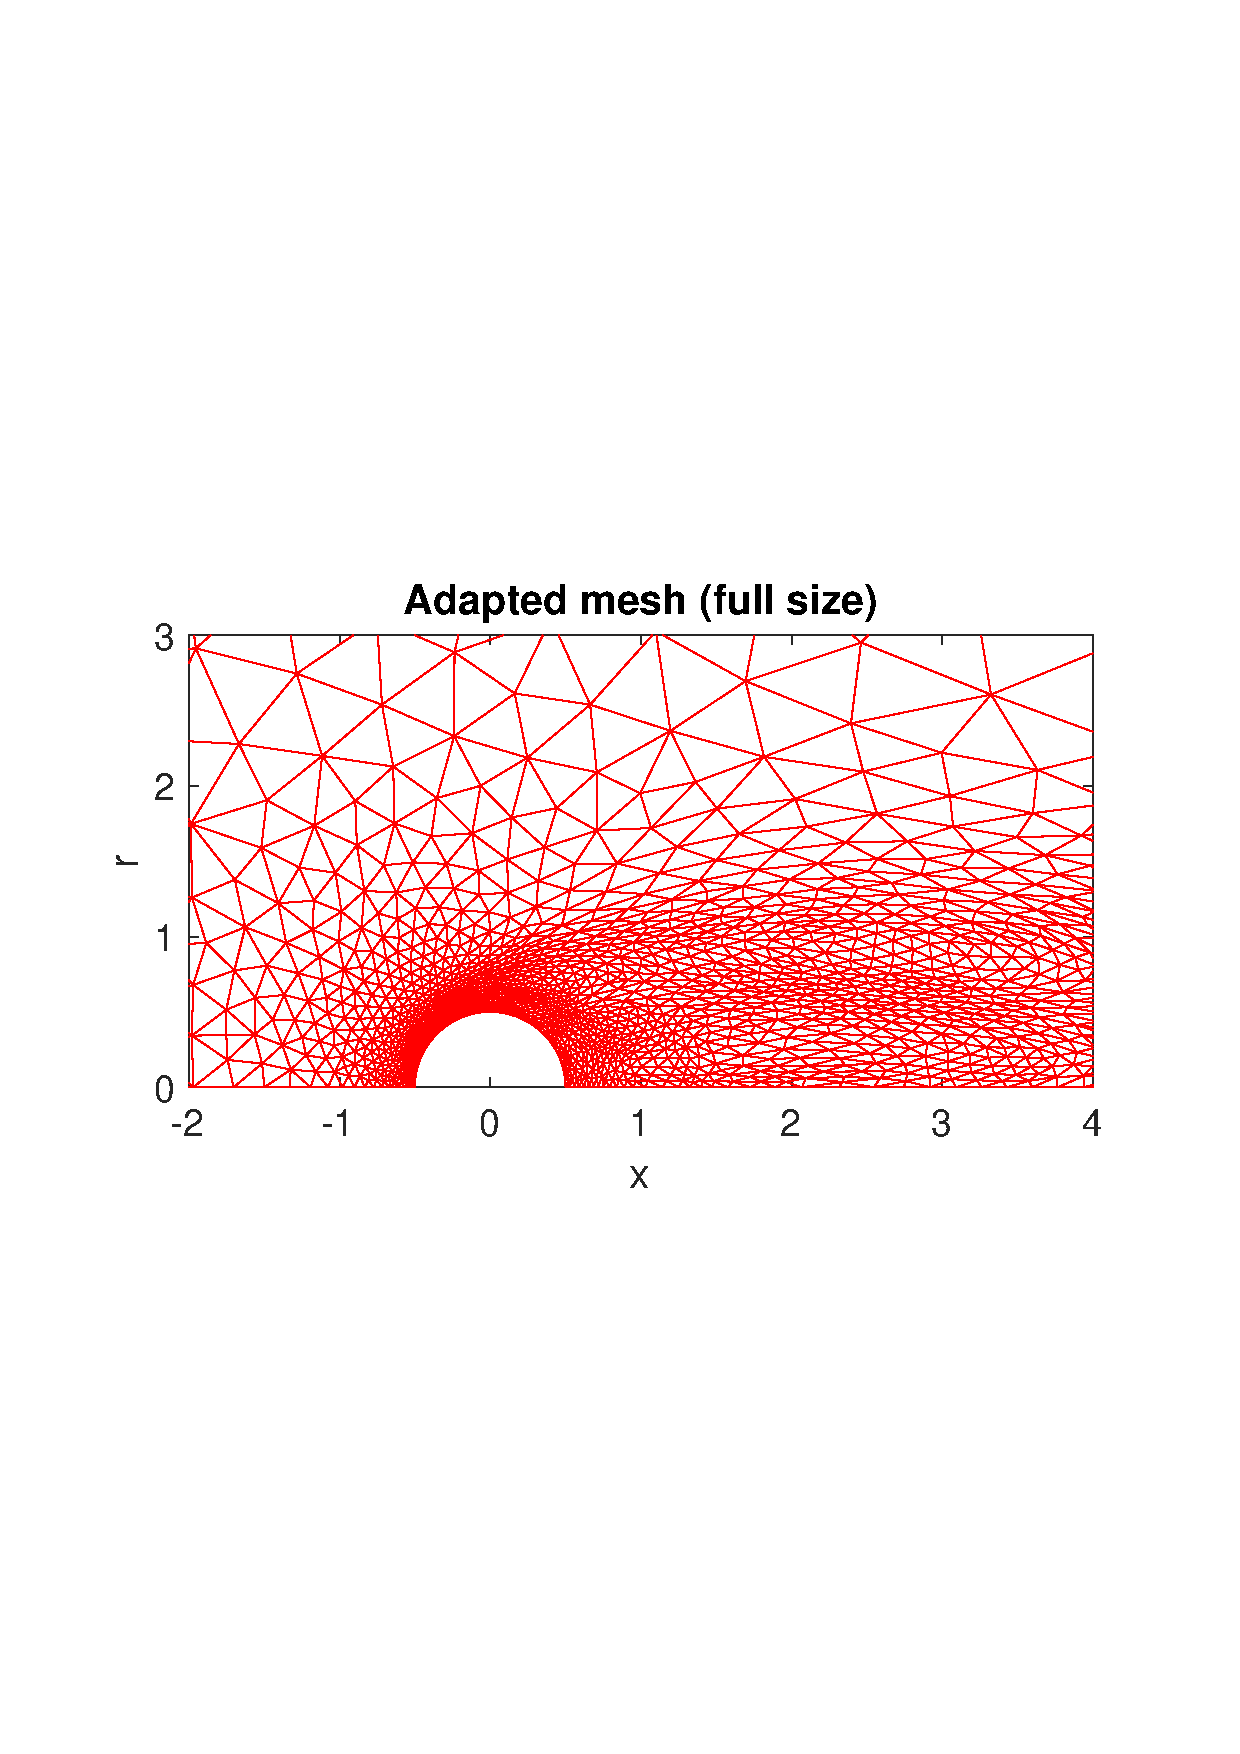
\includegraphics[width=.48 \linewidth]{Cylinder_Mesh.pdf}
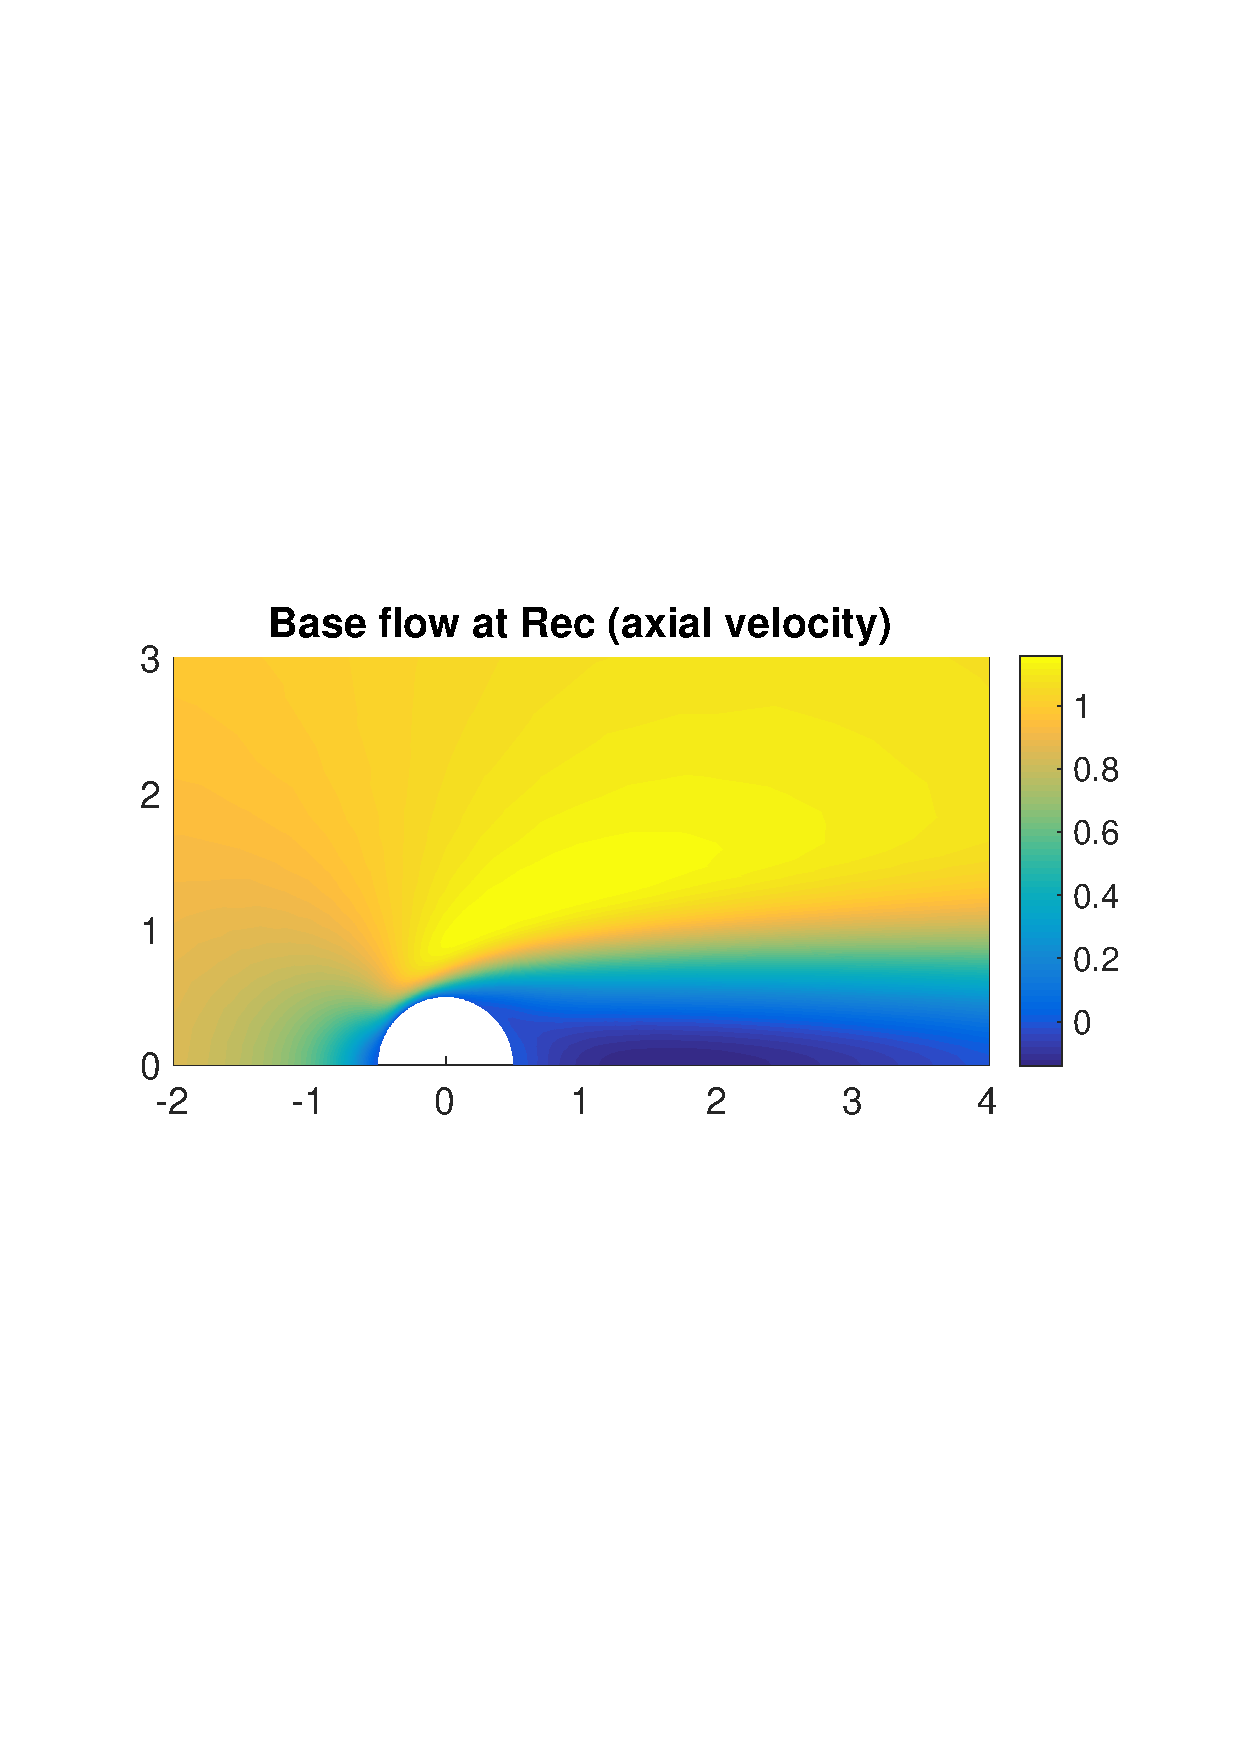
\includegraphics[width=.48 \linewidth]{Cylinder_BaseFlowReC.pdf}
\caption{Adapted mesh $(a)$  and base flow (axial velocity component) ($b$) for the flow over a cylinder at $Re=Re_c = 46.7$.}
\label{fig:Baseflow}
\end{figure}


\paragraph{Base flow characteristics}



%\subsection{Implementation}

%\subsection{Application to the cylinder}

\begin{figure}
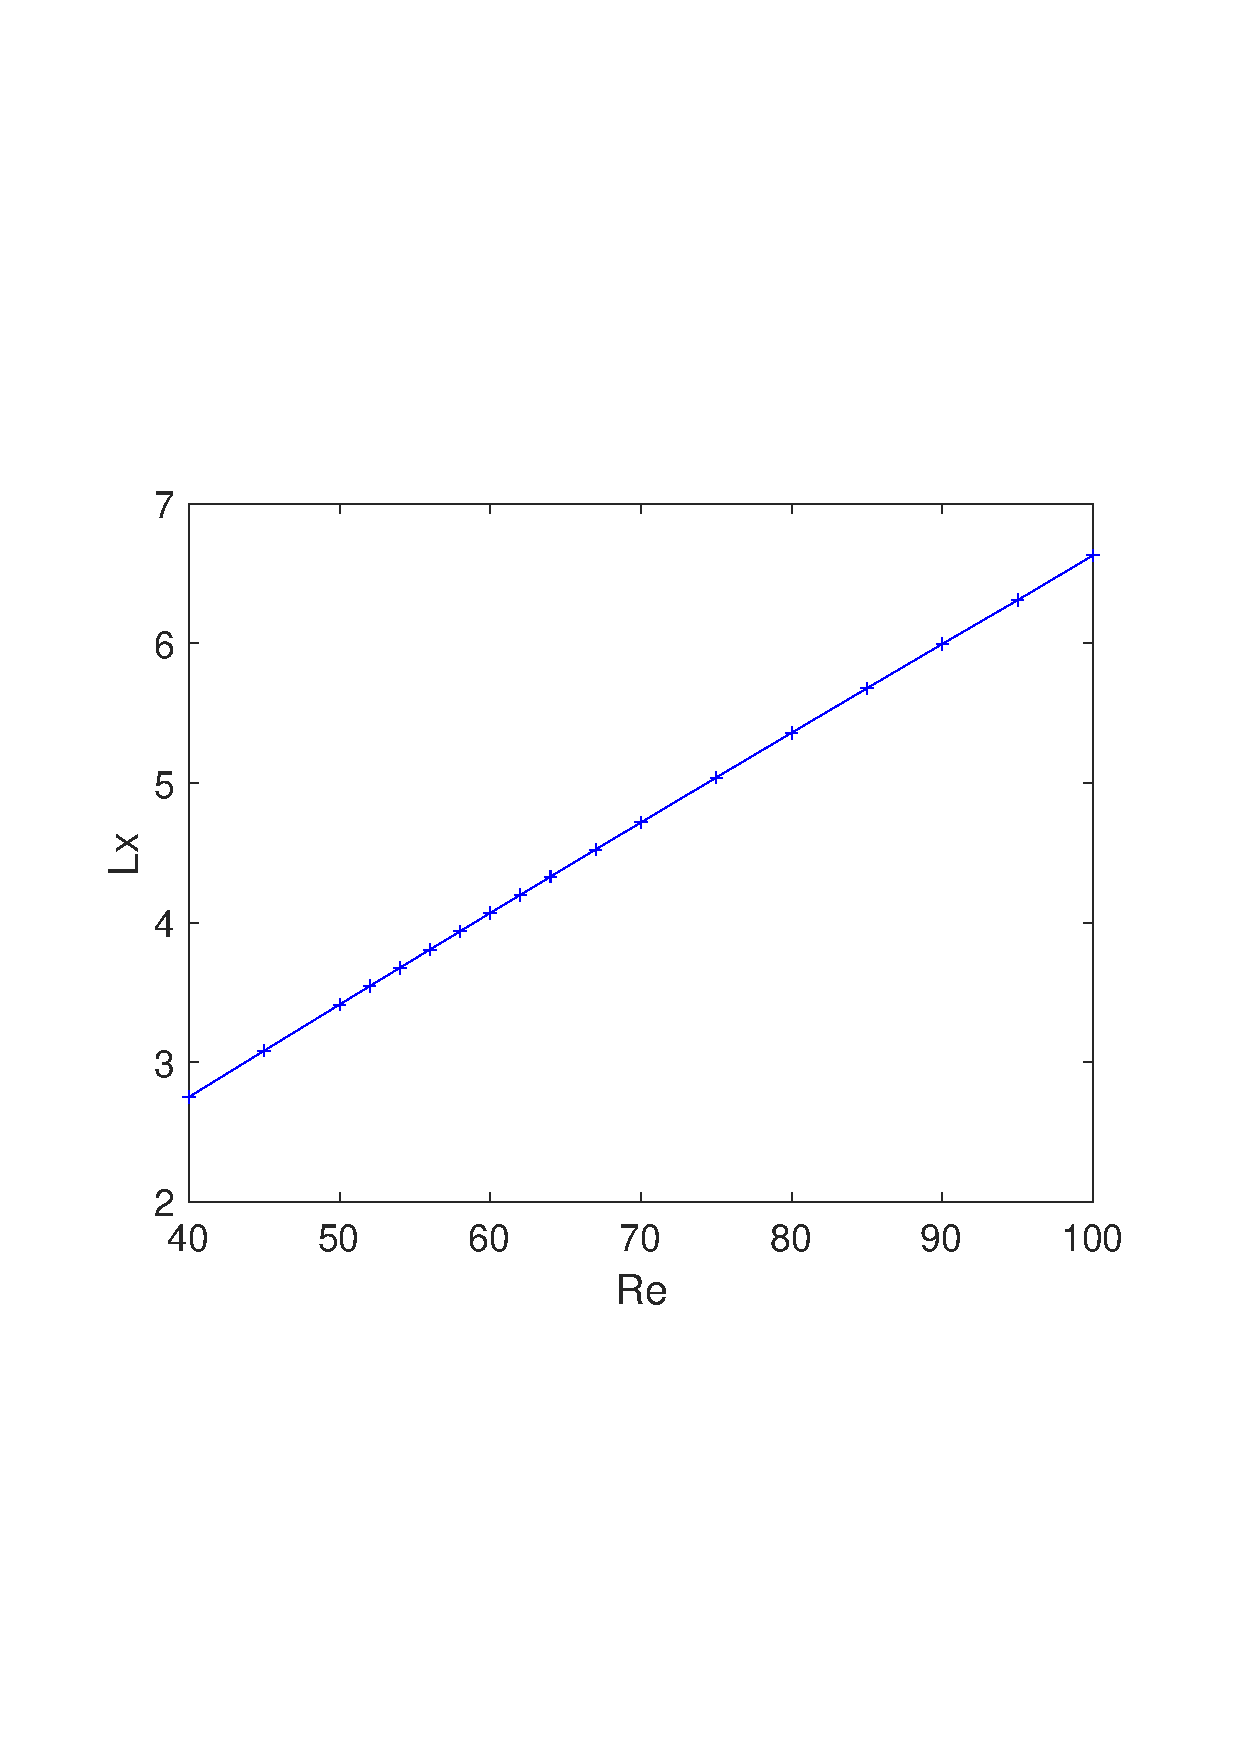
\includegraphics[width=.48 \linewidth]{Cylinder_Lx_baseflow.pdf}
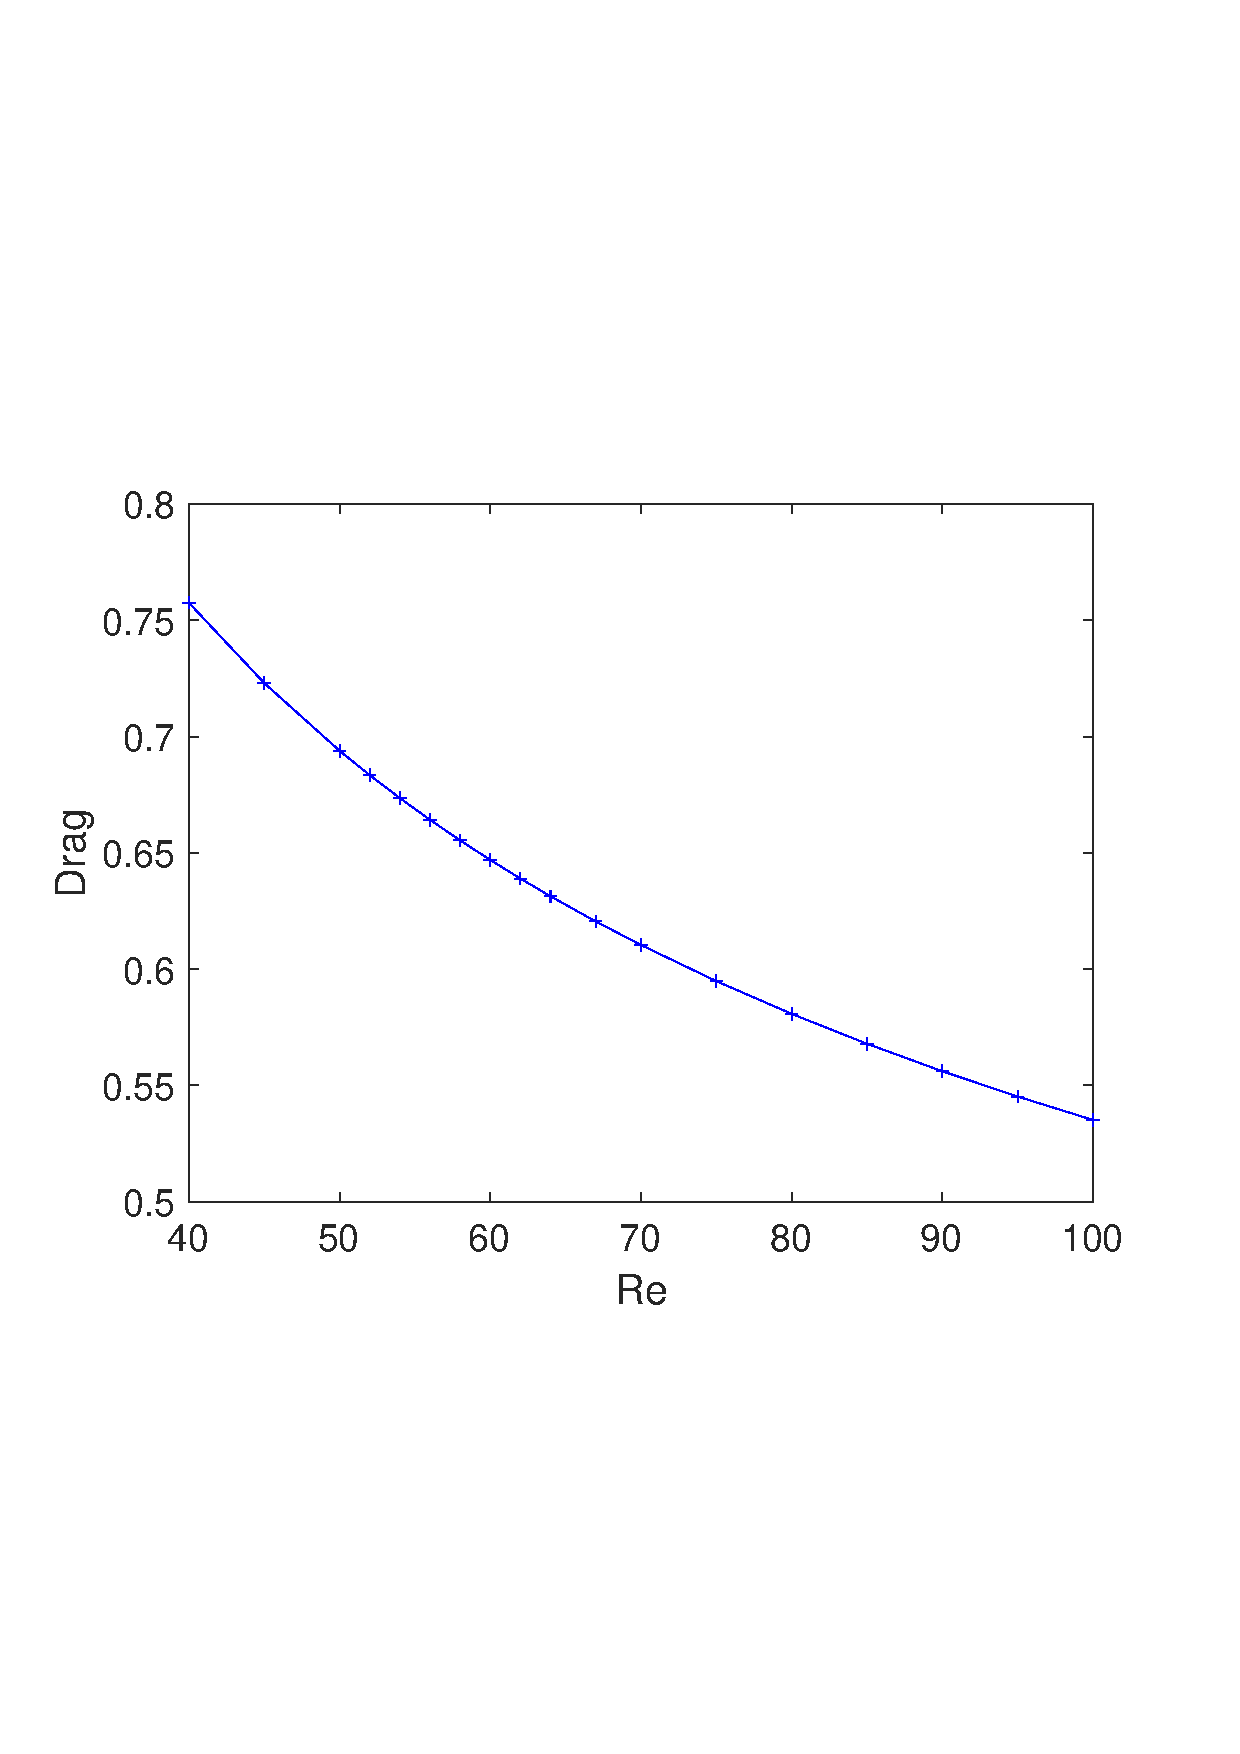
\includegraphics[width=.48 \linewidth]{Cylinder_Drag_baseflow.pdf}
\caption{Recirculation length $L_x$ $(a)$  and drag $C_x$ ($b$) of the base flow over a cylinder at $Re=Re_c = 46.7$.}
\label{fig:LxandDrag}
\end{figure}

\clearpage

\section{Computing an eigenmode with a shift-invert method}

We consider the stability using the classical ansatz 

${\bf u} = {\bf u}_b + \hat{{\bf u}} e^{\lambda t}$

Where $\lambda = \sigma + i \omega$ is the eigenvalue, $\sigma$ the amplification rate,
$\omega$ the oscillation rate, $\hat{{\bf u}}$ the eigenmode.

The eigenmode is governed by the linear problem



After discretization we end up 




\paragraph{Stability equations}

Eigenvalue problem

Adjoint eigenvalue problem

Sensitivity

\paragraph{Iterative methods}

These de Andrea Fani



\paragraph{Implementation}

Matlab driver...


\subsection{Results}

\begin{figure}
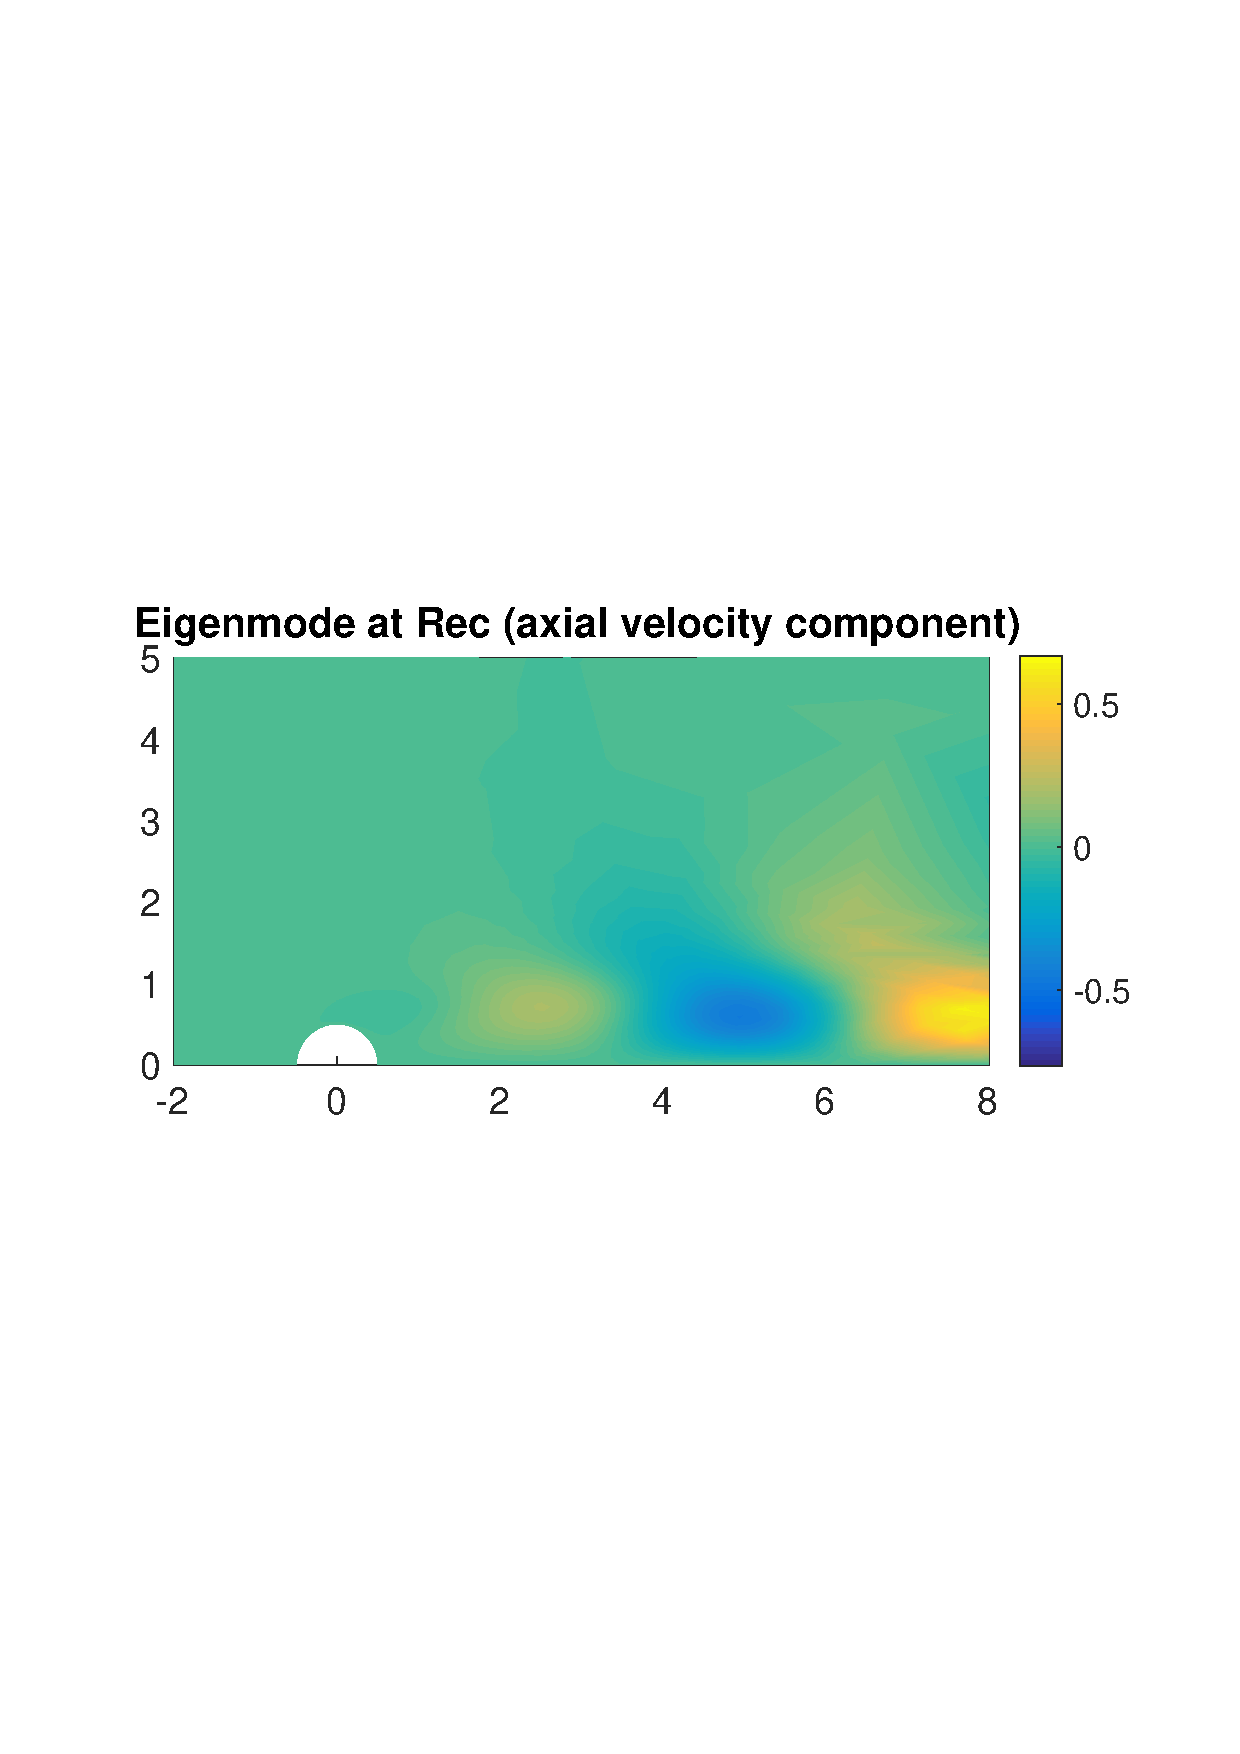
\includegraphics[width=.48 \linewidth]{Cylinder_EigenModeReC.pdf}
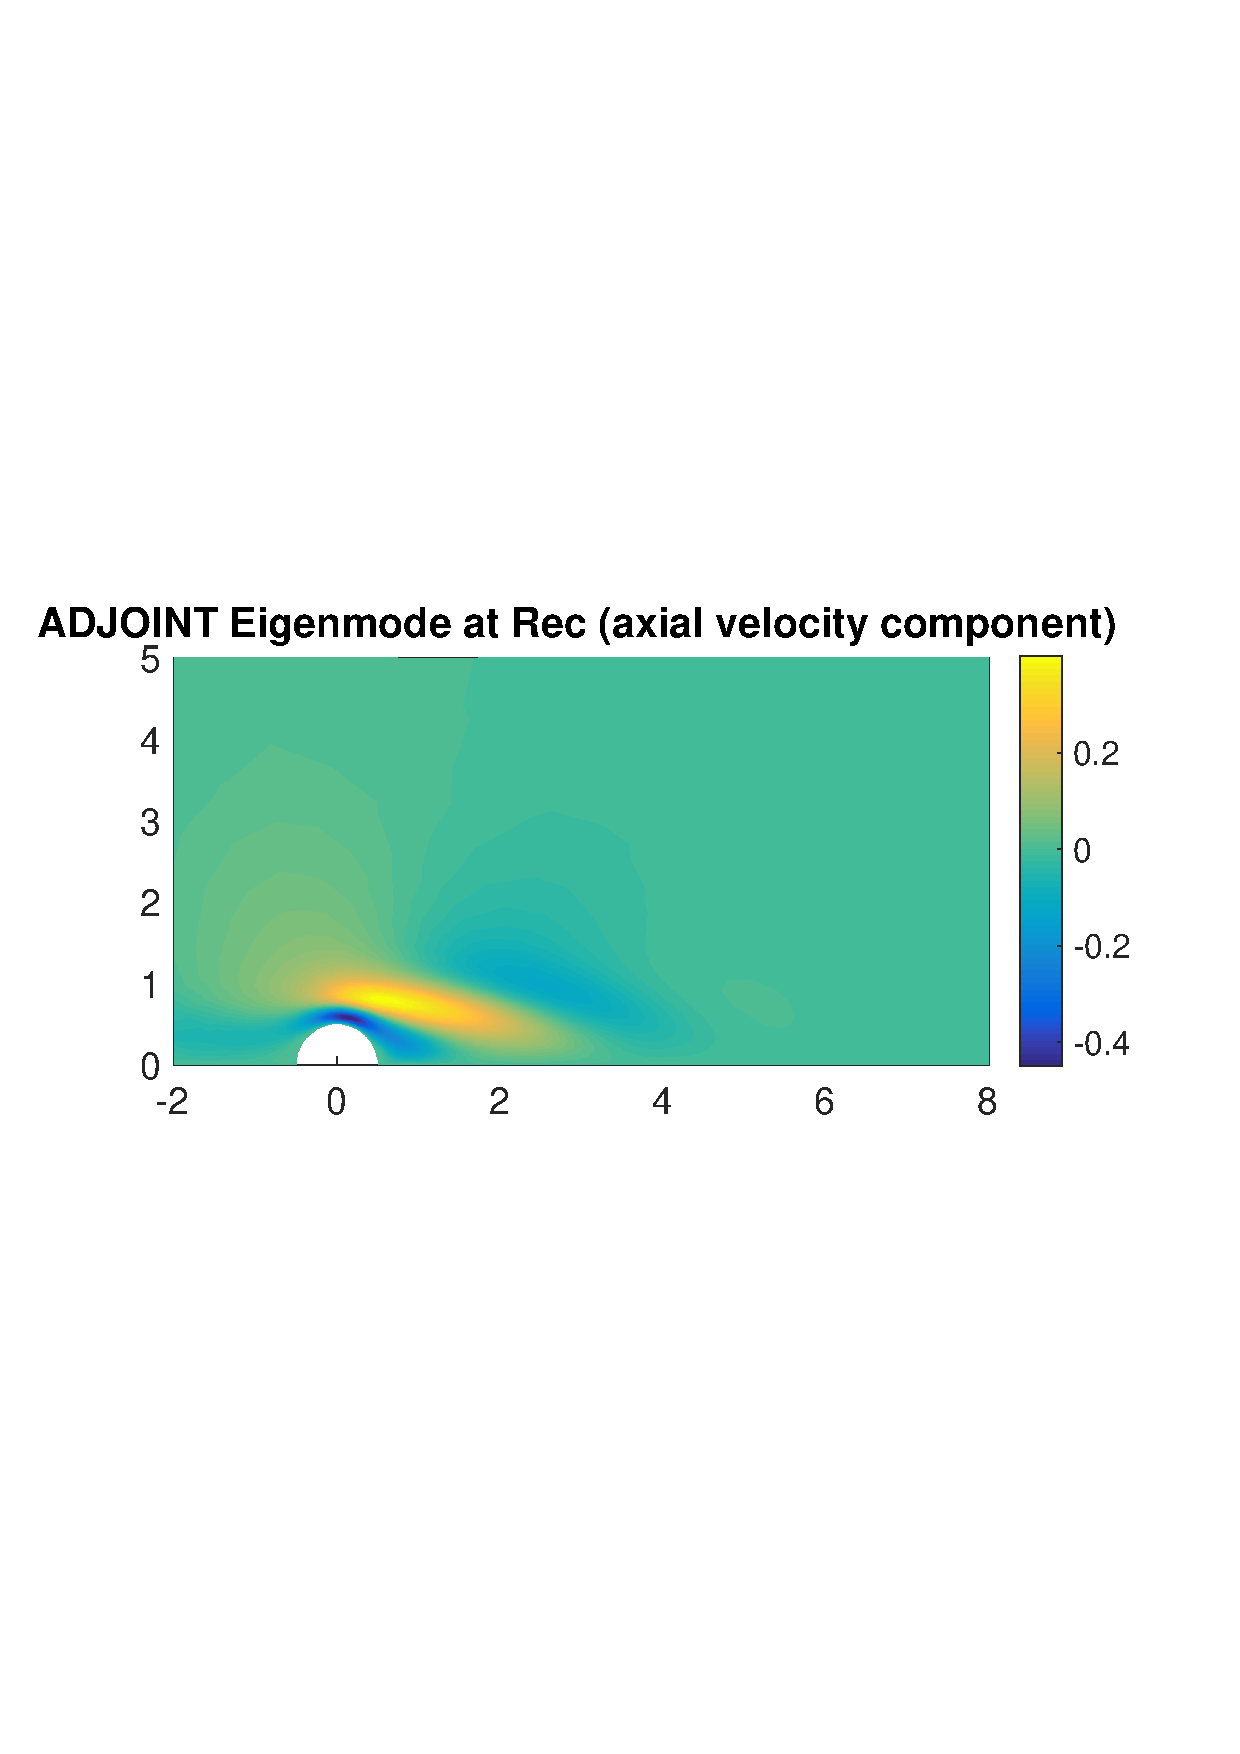
\includegraphics[width=.48 \linewidth]{Cylinder_EigenModeAdjReC.pdf}
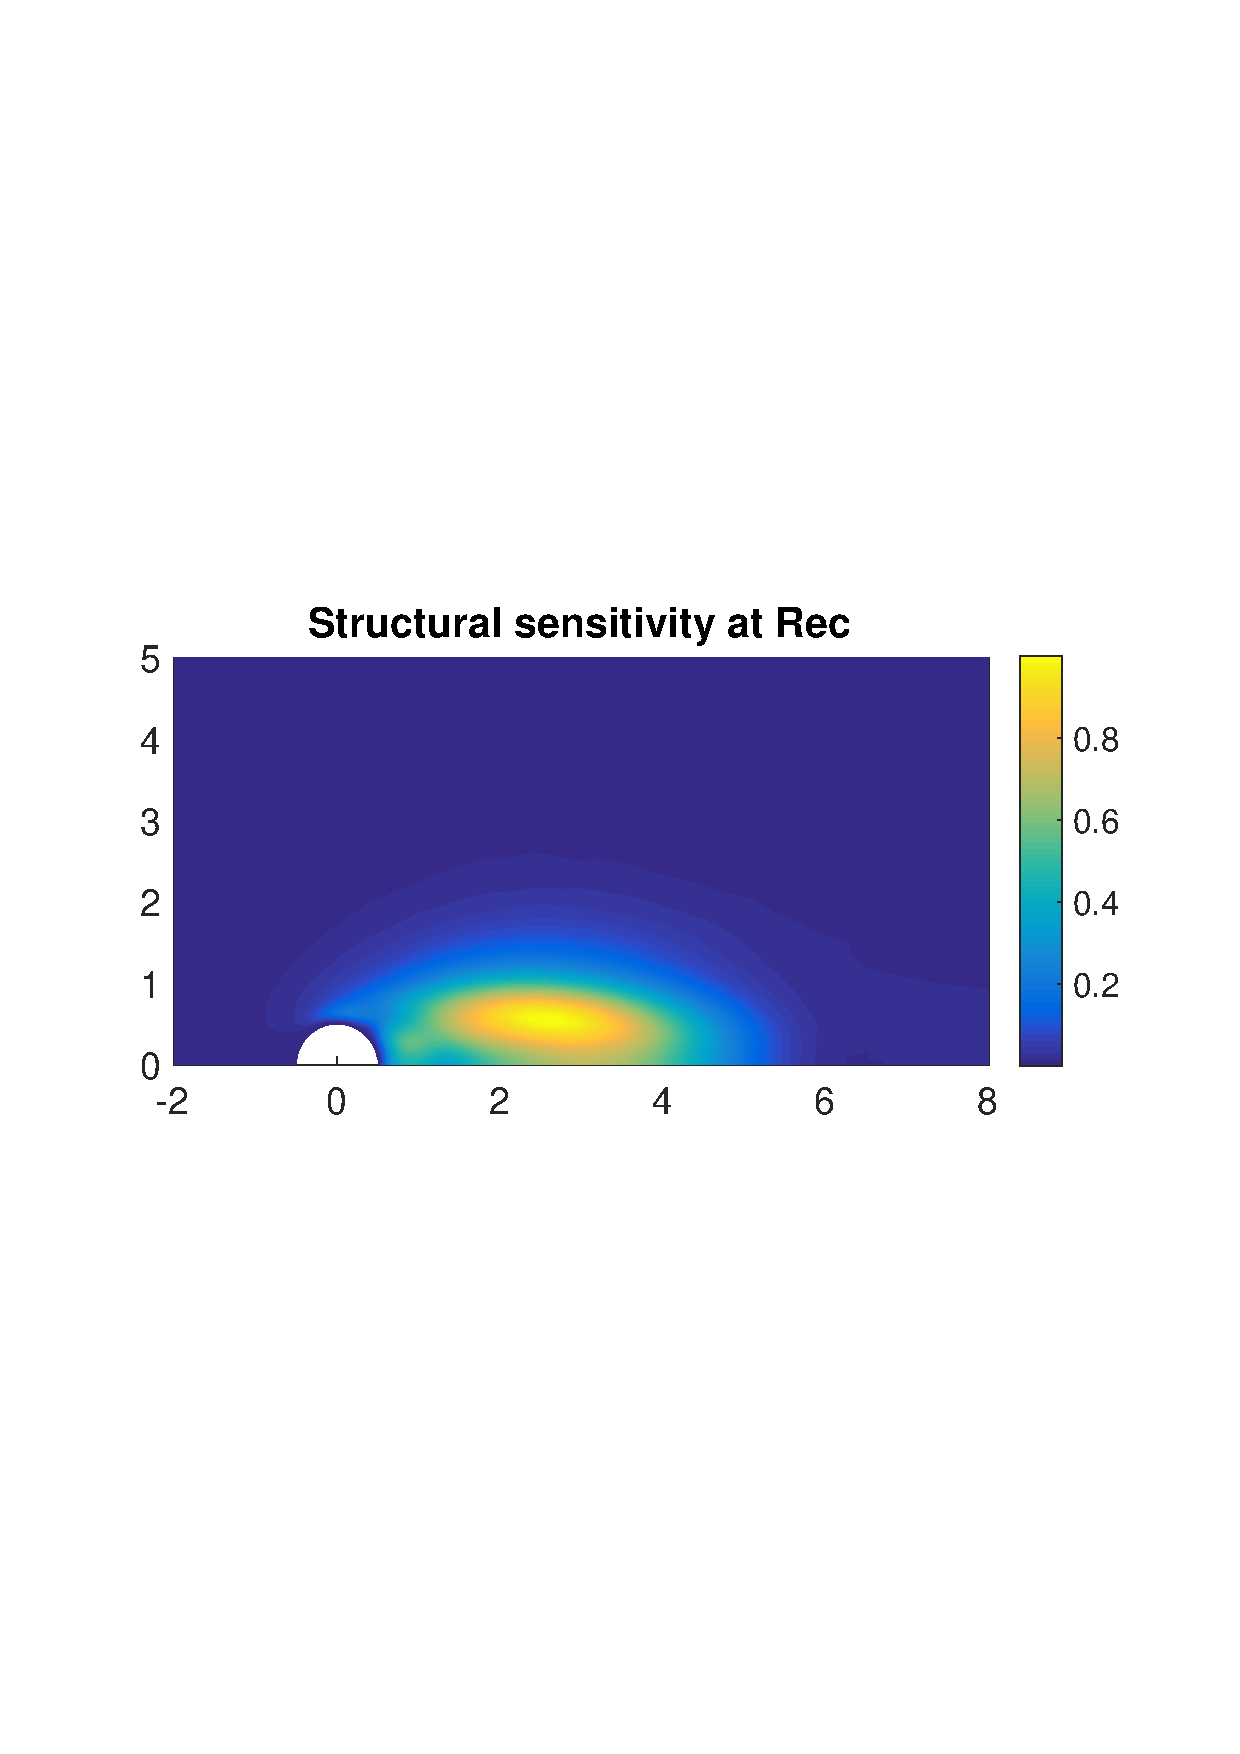
\includegraphics[width=.48 \linewidth]{Cylinder_SensitivityReC.pdf}
\caption{Eigenmode $(a)$  (axial velocity component),  Adjoint eigenmode $(b)$ and structural sensitivity ($c$) for the cylinder's wake at $Re=Re_c = 46.7$.}
\label{fig:Eigenmode}
\end{figure}


\begin{figure}
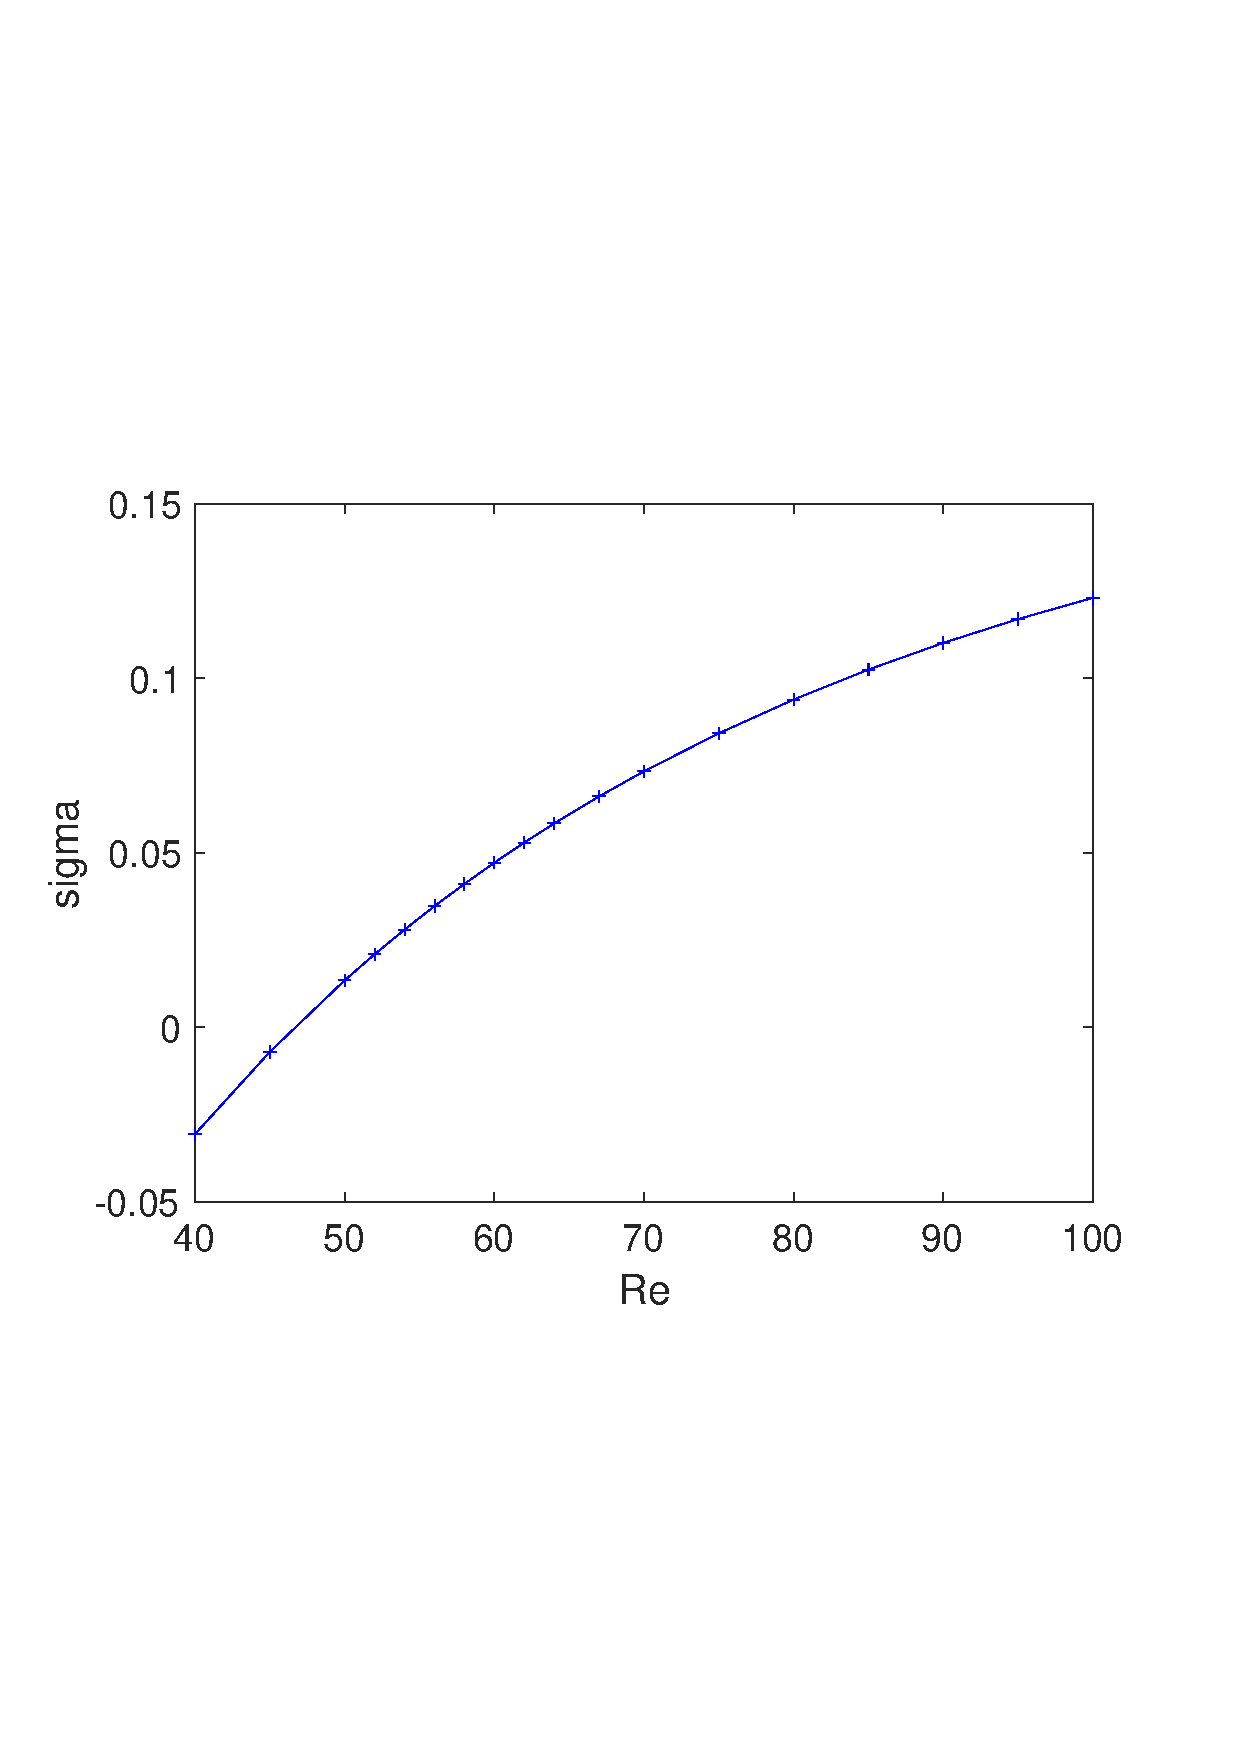
\includegraphics[width=.48 \linewidth]{Cylinder_Sigma_Re.pdf}
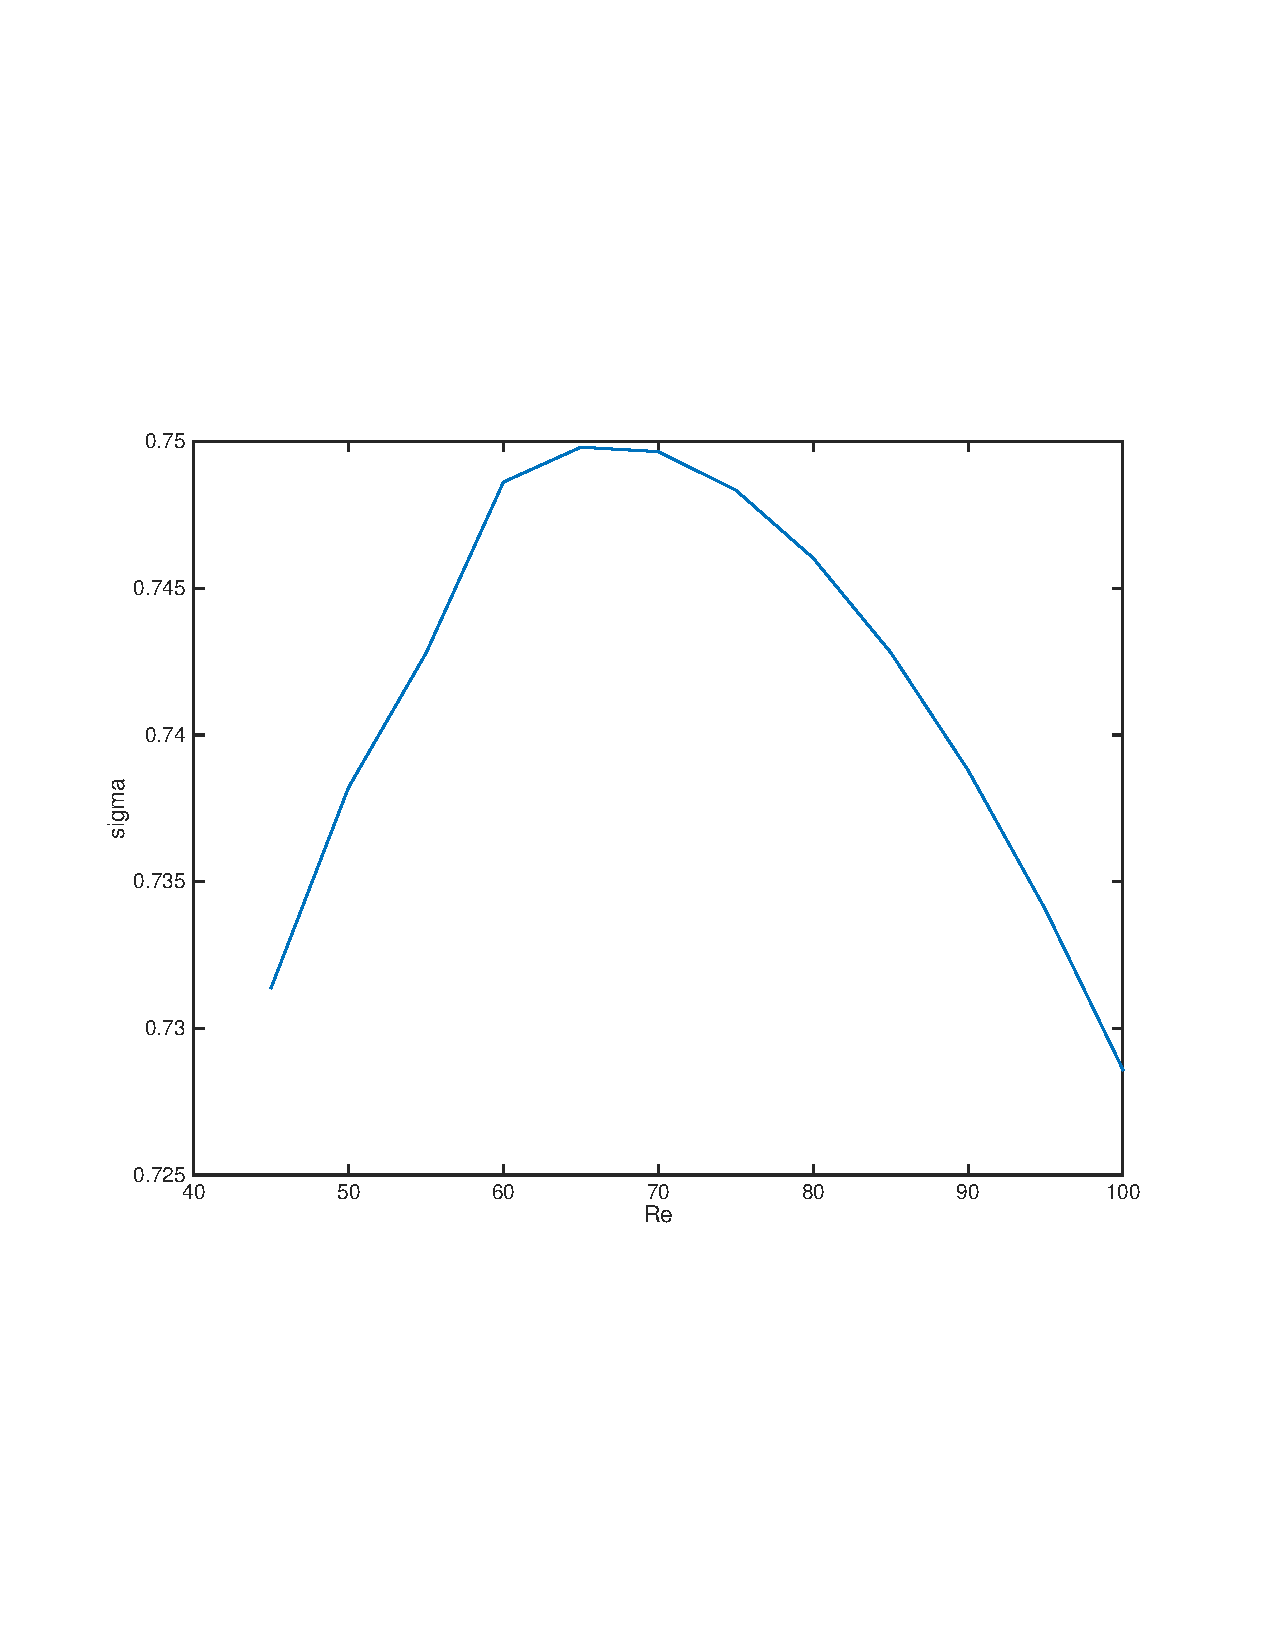
\includegraphics[width=.48 \linewidth]{Cylinder_Omega_Re.pdf}
\caption{Growth rate $\sigma$ $(a)$  and Strouhal number $St = (a \omega)/(2\pi U_0)$ ($b$) as function of Reynolds number}
\label{fig:SigmaOmega}
\end{figure}


\subsection{Application}

\section{Computing the limit cycle for $Re>Re_c$ with Harmonic Balance}


\begin{figure}
\begin{center}
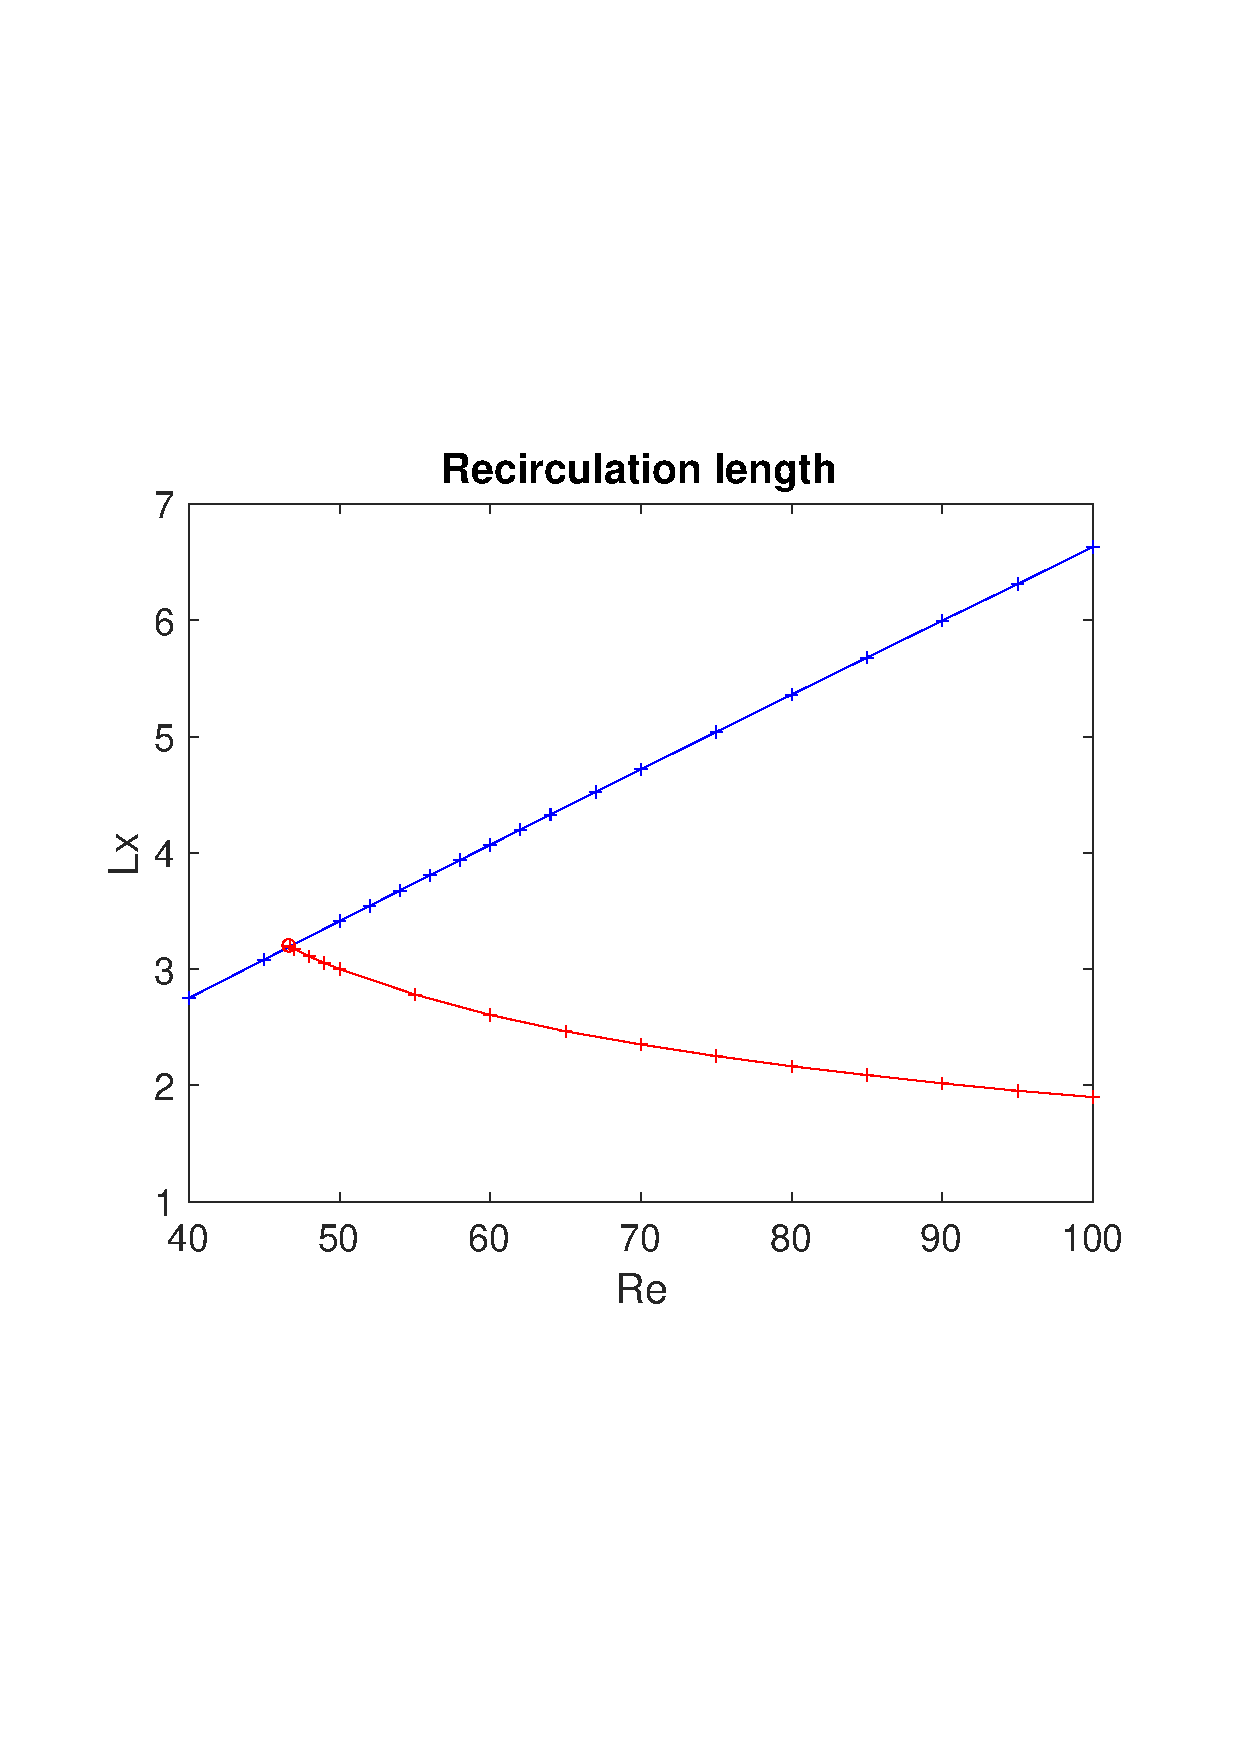
\includegraphics[width=.48 \linewidth]{Cylinder_Lx_Re_SC.pdf}
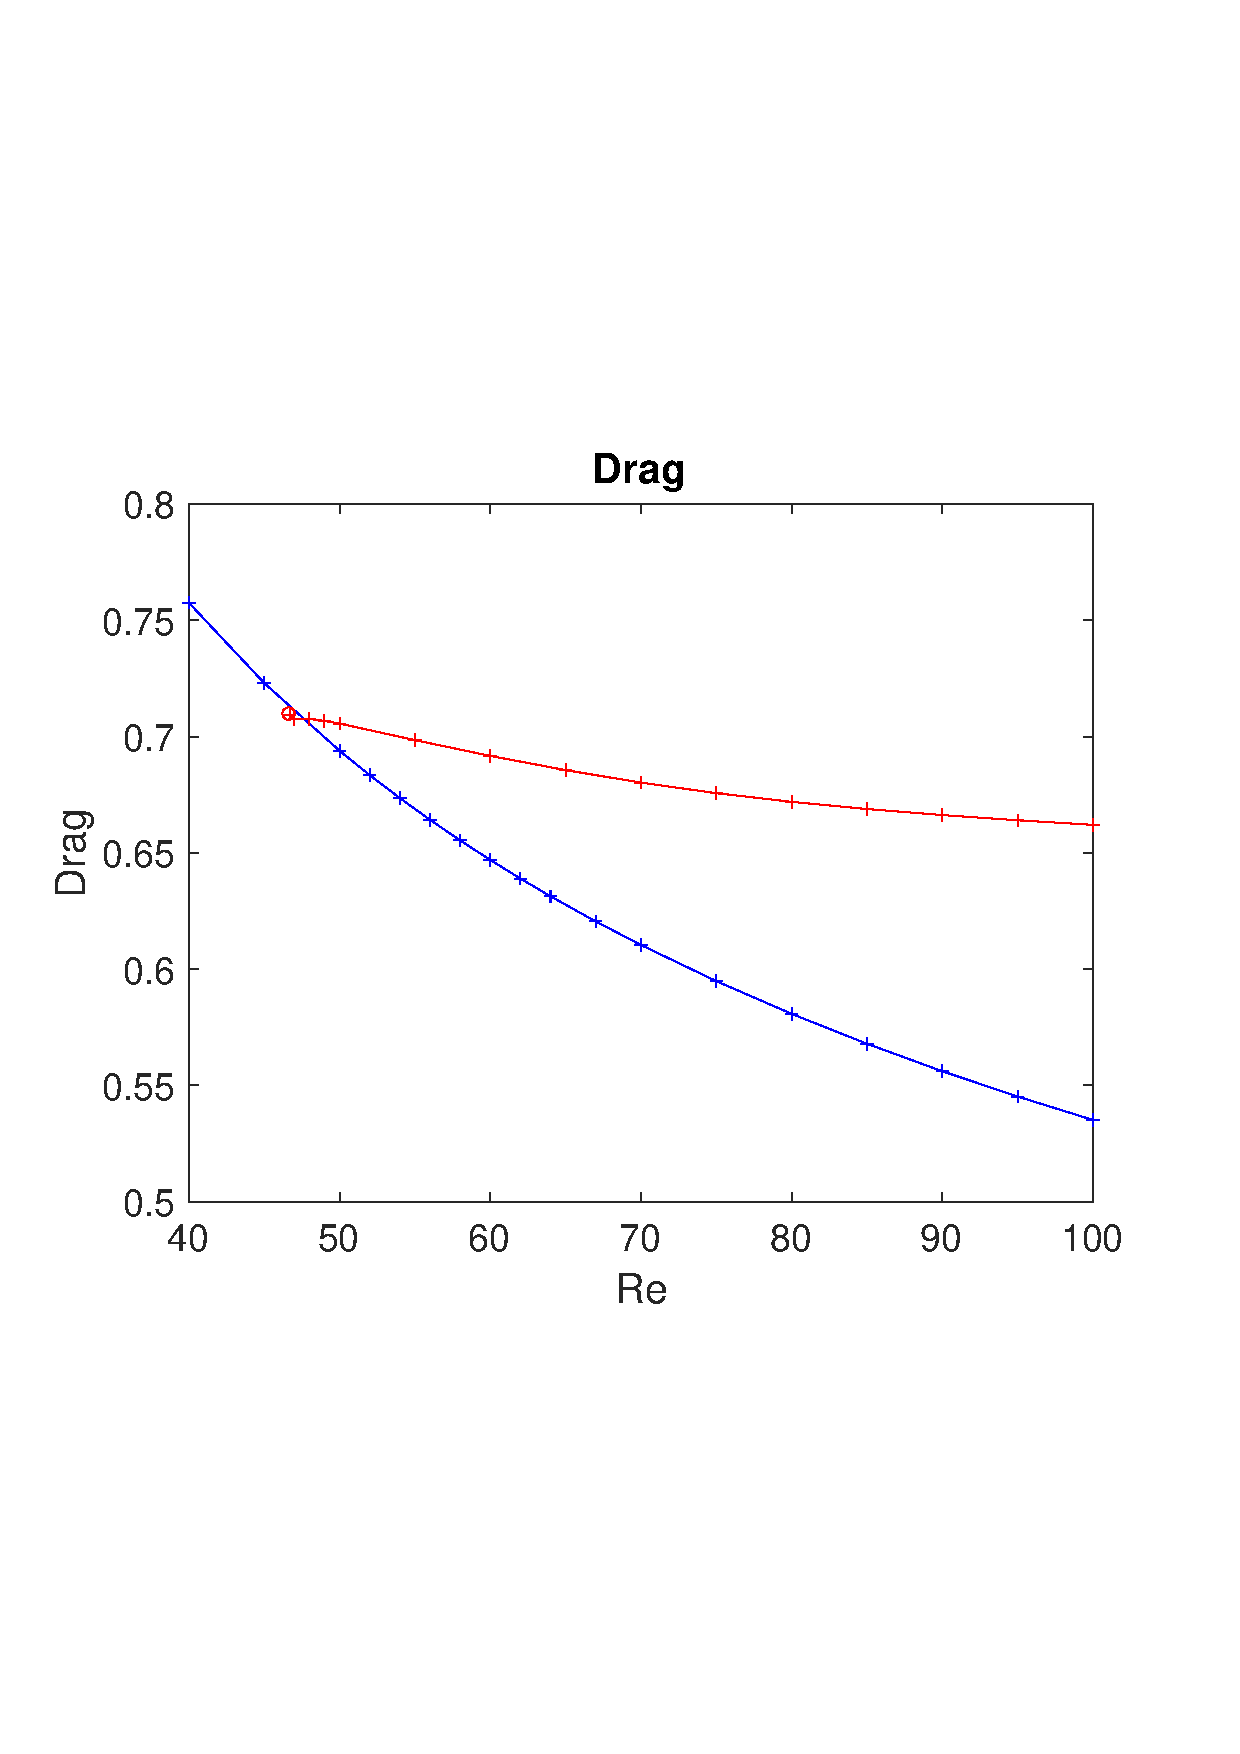
\includegraphics[width=.48 \linewidth]{Cylinder_Drag_Re_SC.pdf}
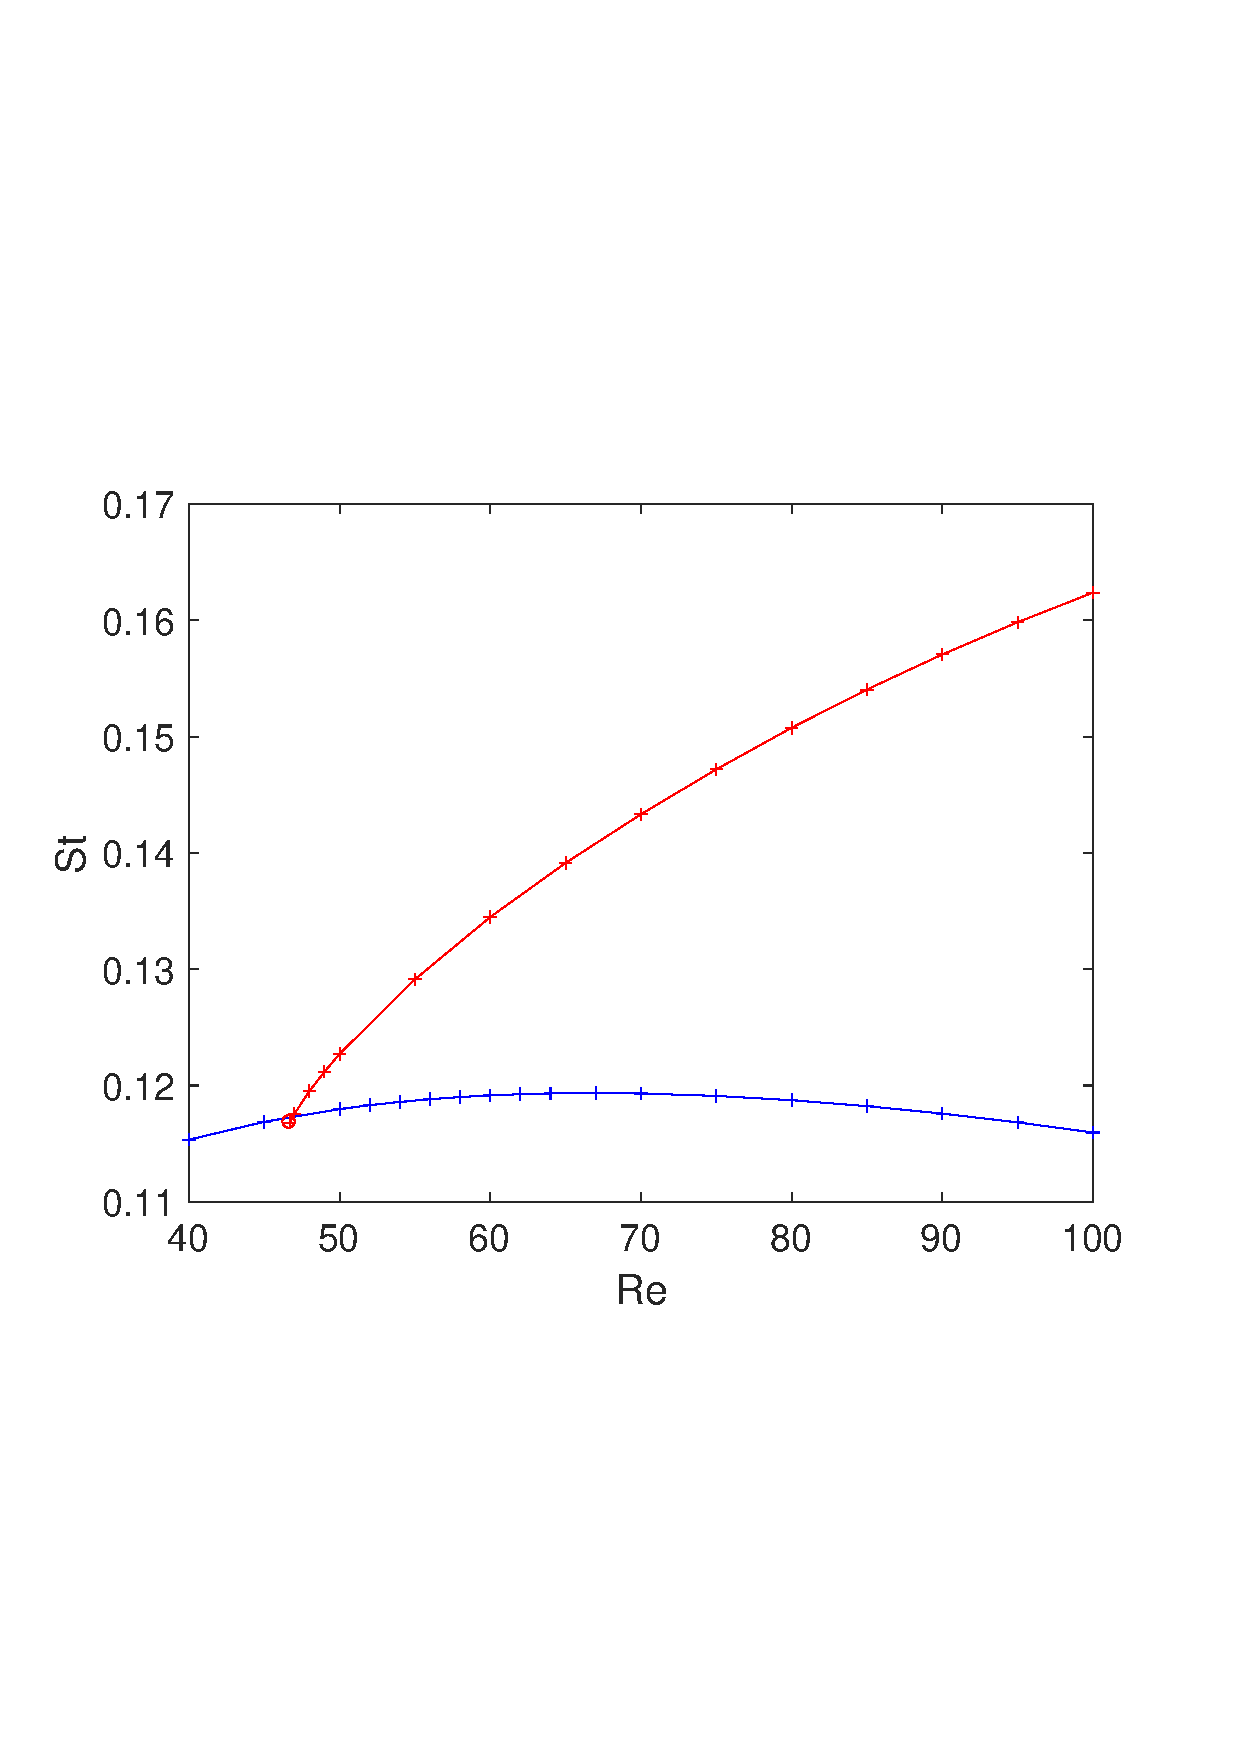
\includegraphics[width=.48 \linewidth]{Cylinder_Omega_Re_SC.pdf}
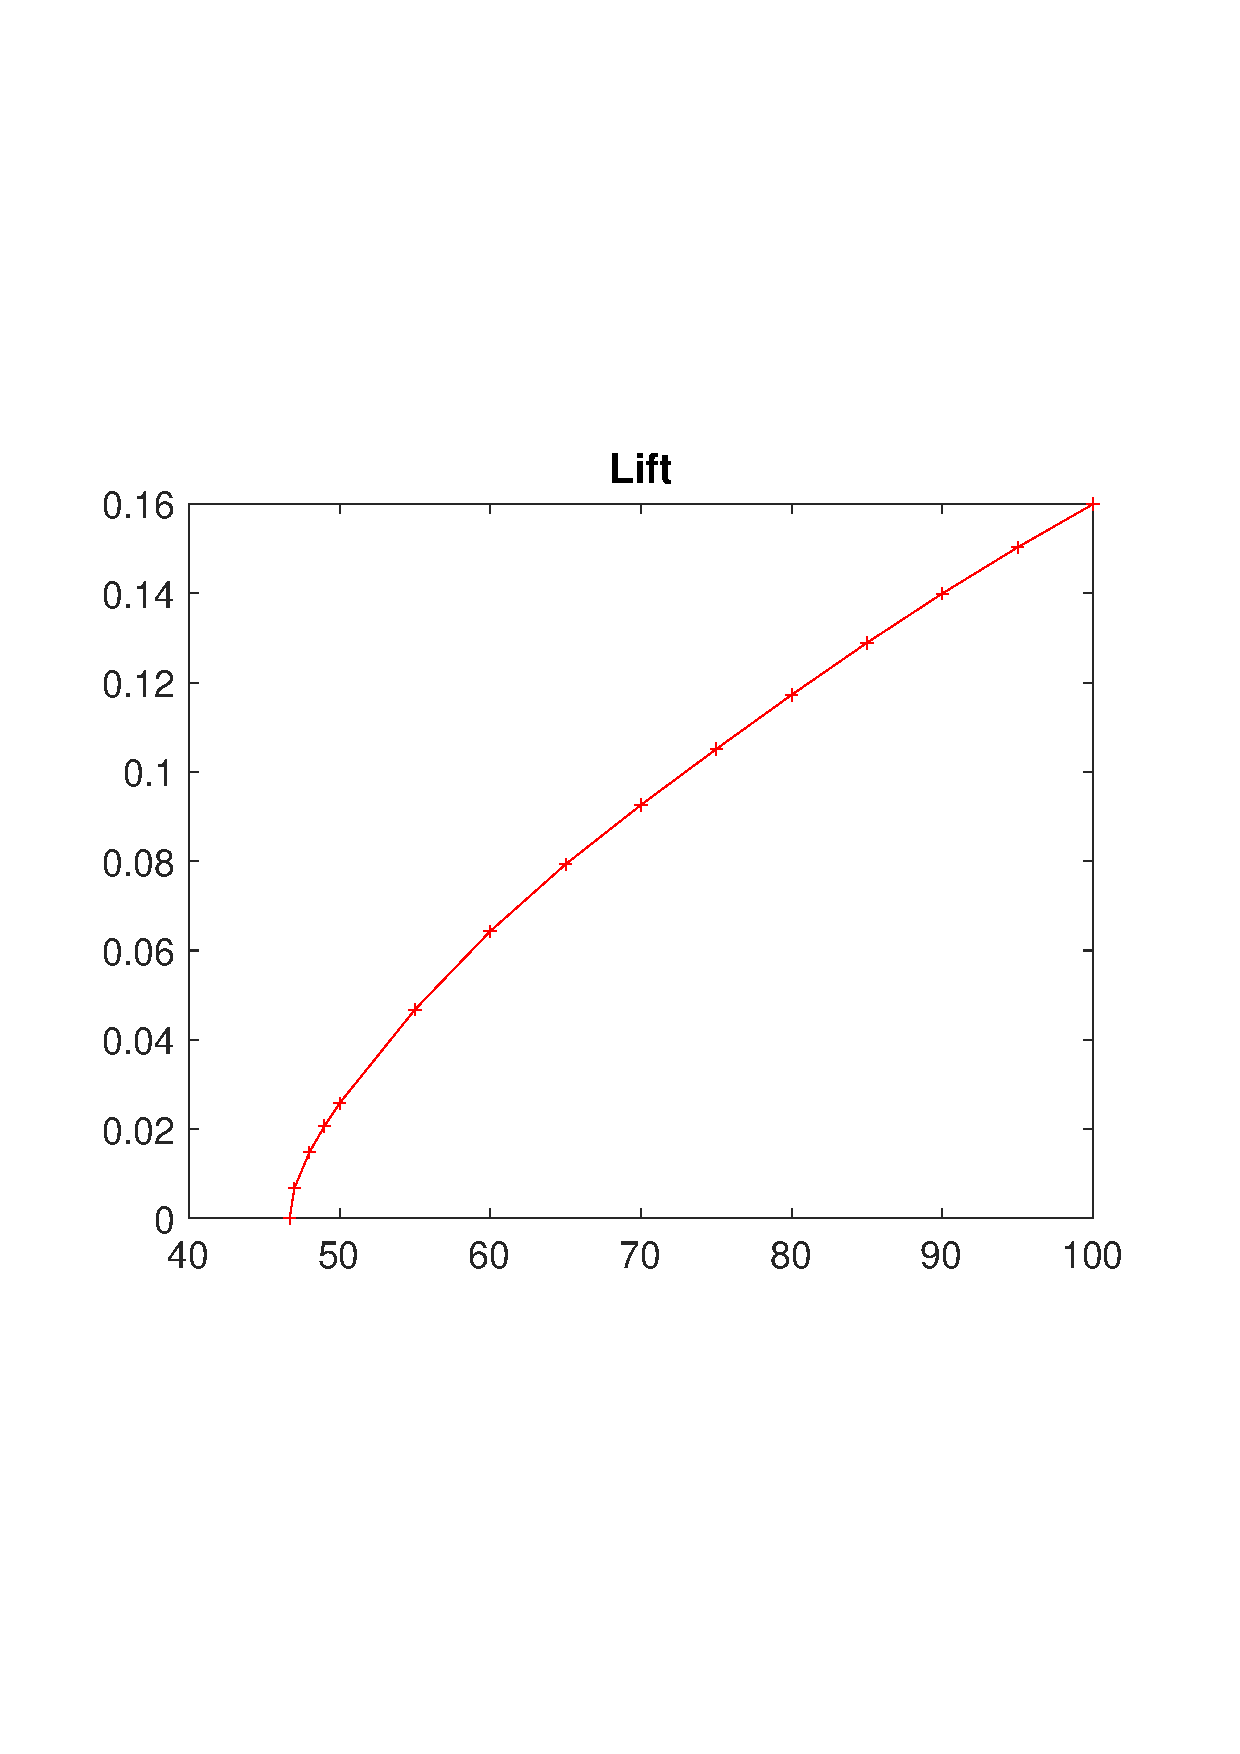
\includegraphics[width=.48 \linewidth]{Cylinder_Lift_Re_SC.pdf}
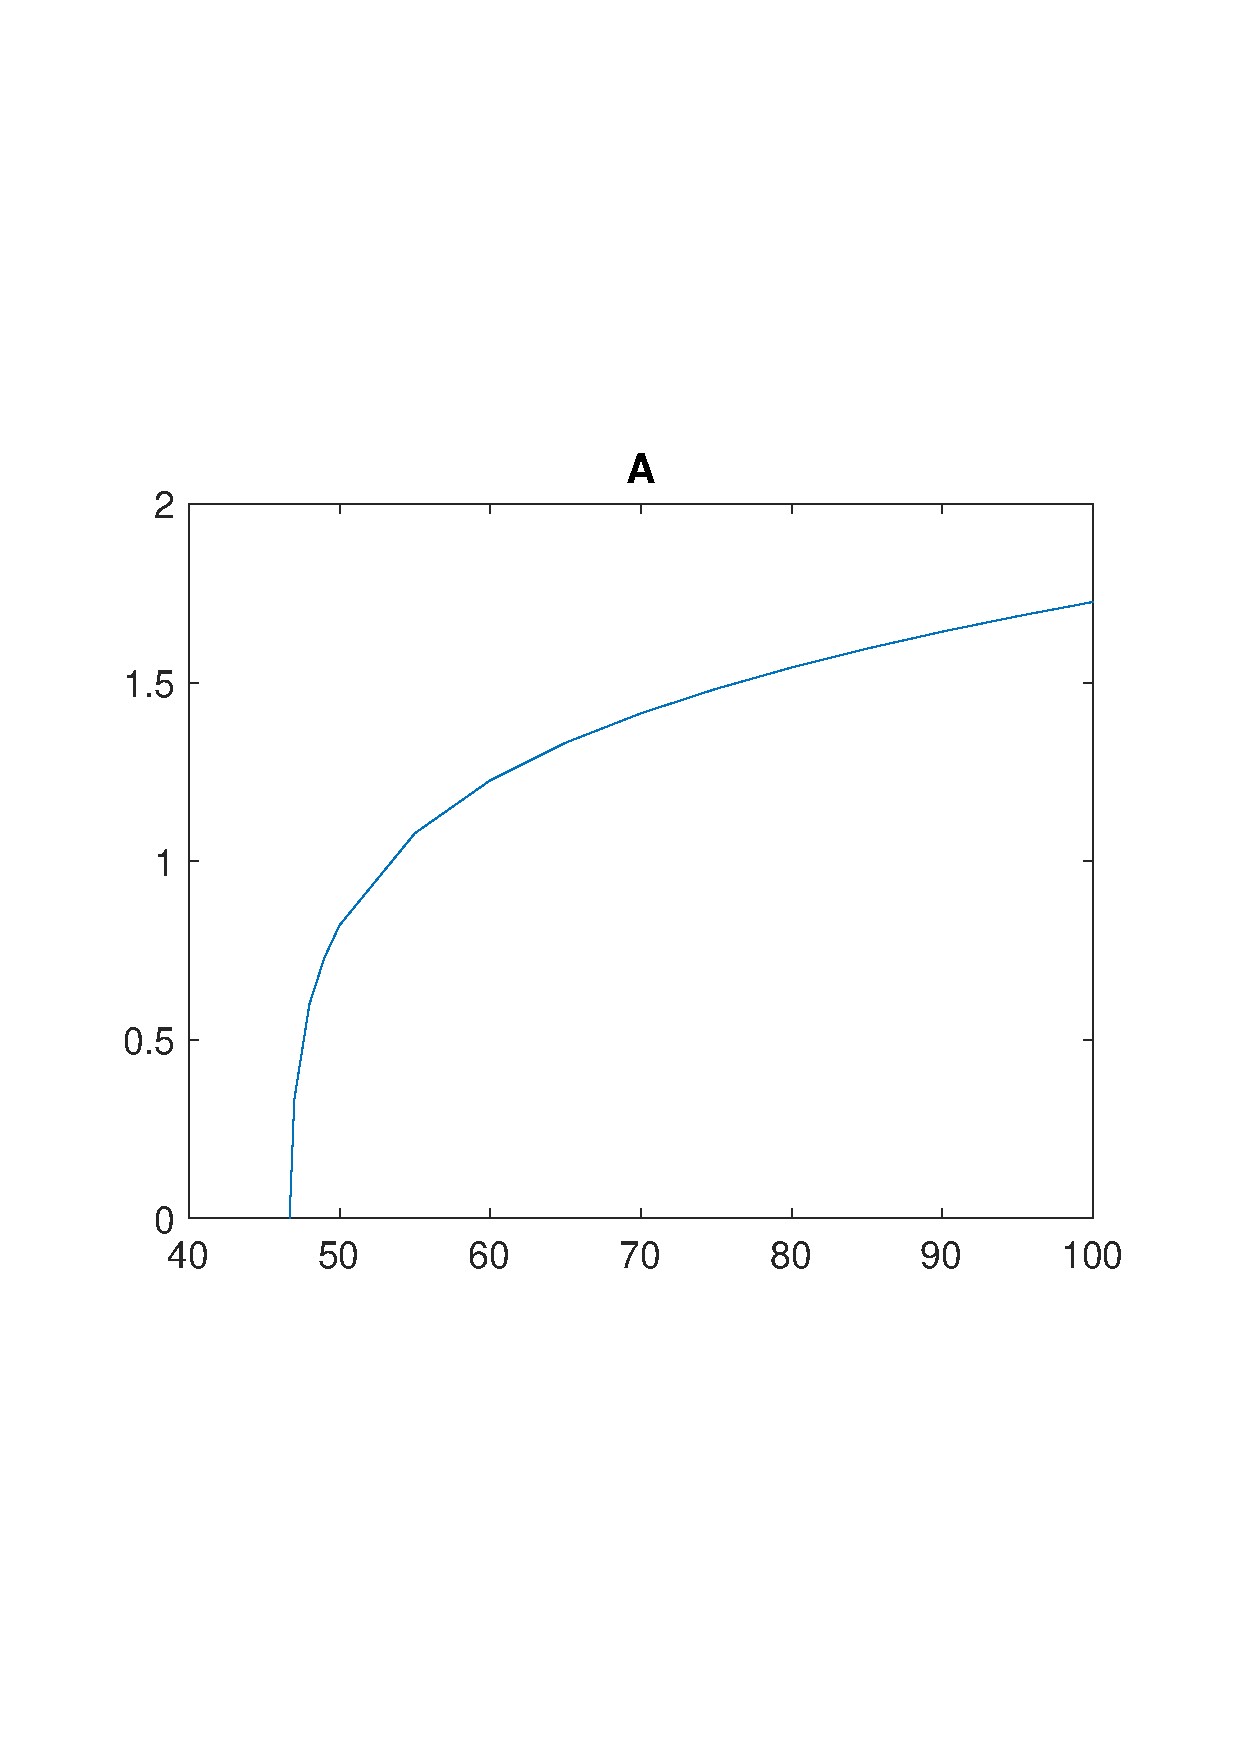
\includegraphics[width=.48 \linewidth]{Cylinder_Energy_Re_SC.pdf}
\end{center}
\caption{HARMONIC BALANCE APPROACH FOR THE WAKE OF A CYLINDER}
\label{fig:HB}
\end{figure}


\begin{figure}
\begin{center}
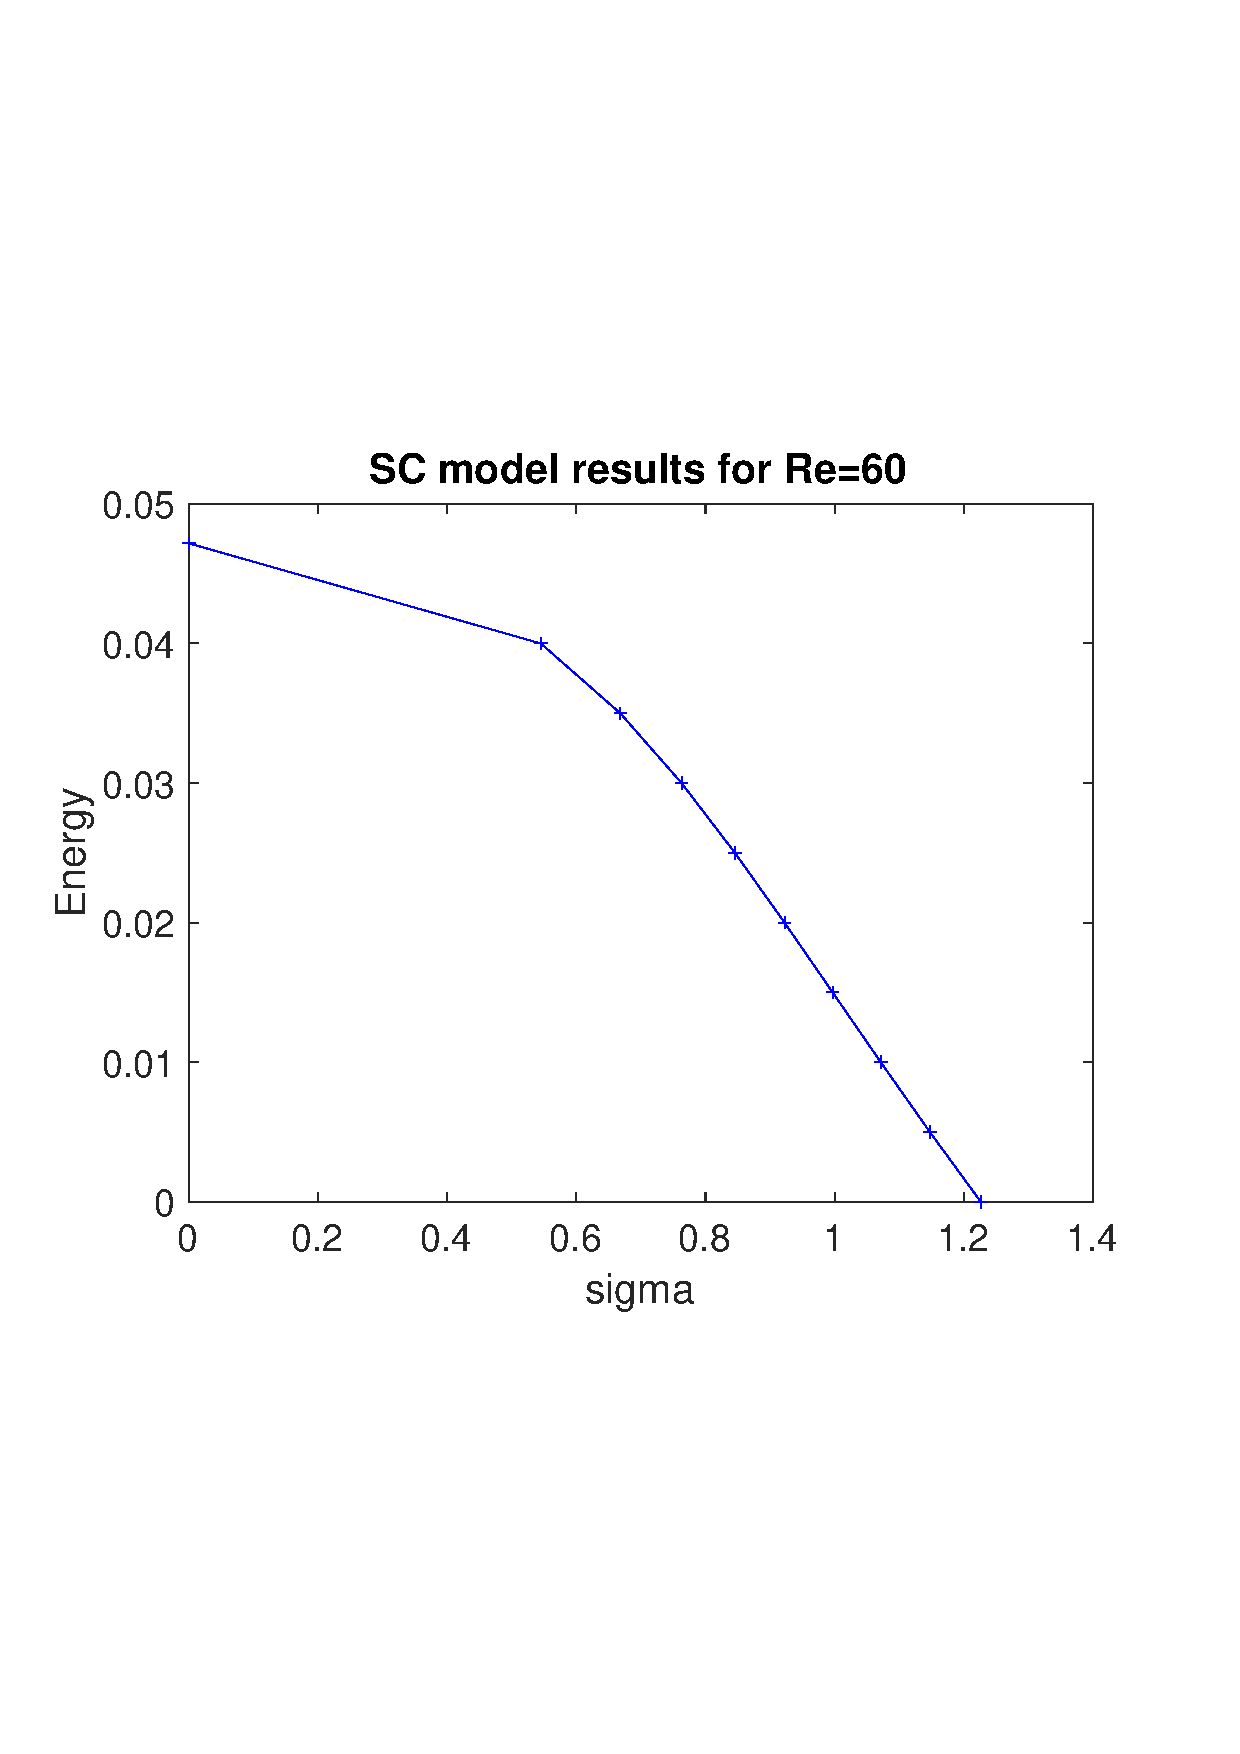
\includegraphics[width=.48 \linewidth]{Cylinder_SC60_EnergySigma.pdf}
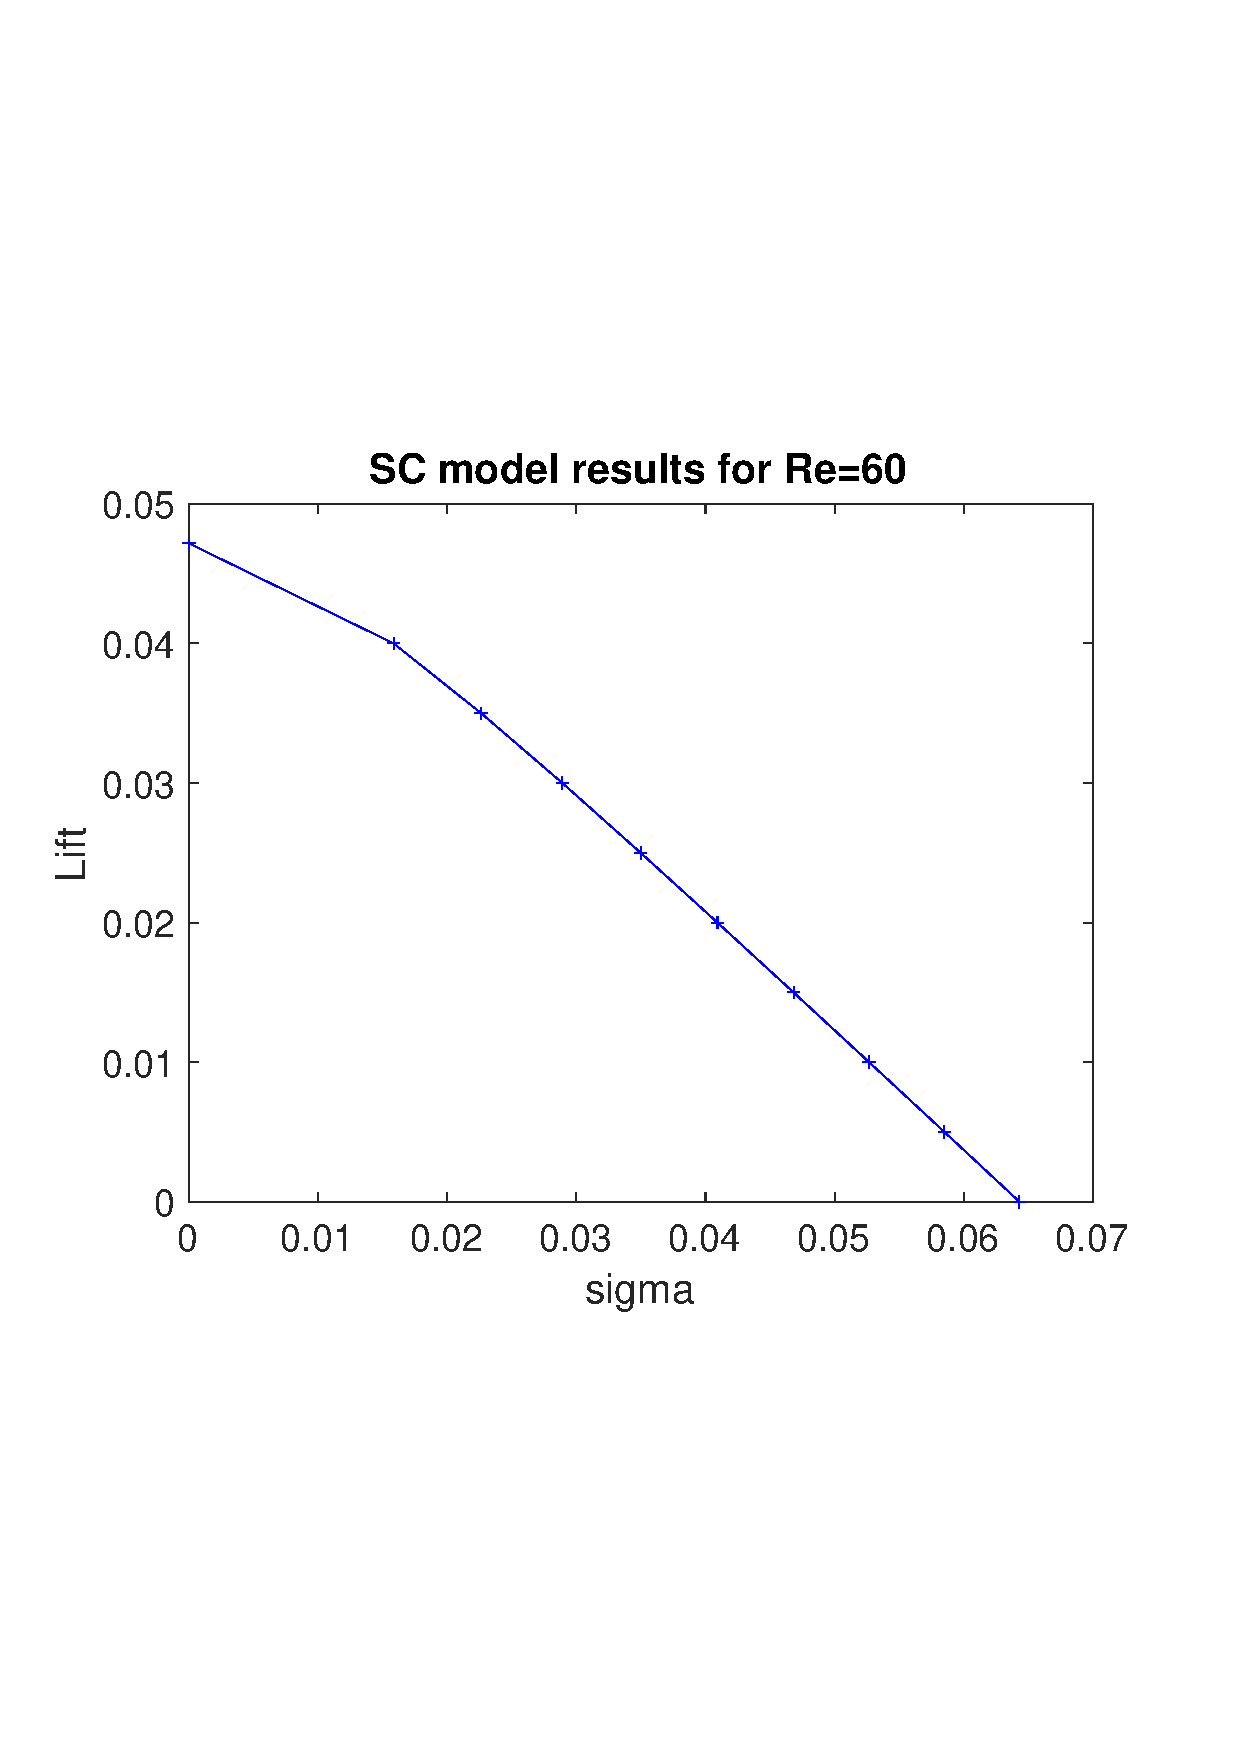
\includegraphics[width=.48 \linewidth]{Cylinder_SC60_LiftSigma.pdf}
\end{center}
\caption{SELF CONSISTENT APPROACH FOR THE WAKE OF A CYLINDER, $Re = 60$}
\label{fig:SC60}
\end{figure}






\appendix

\section{Appendix : details on mesh convergence}


\end{document}



\paragraph{Installation} If the document class \emph{elsarticle} is not available on your computer, you can download and install the system package \emph{texlive-publishers} (Linux) or install the \LaTeX\ package \emph{elsarticle} using the package manager of your \TeX\ installation, which is typically \TeX\ Live or Mik\TeX.

\paragraph{Usage} Once the package is properly installed, you can use the document class \emph{elsarticle} to create a manuscript. Please make sure that your manuscript follows the guidelines in the Guide for Authors of the relevant journal. It is not necessary to typeset your manuscript in exactly the same way as an article, unless you are submitting to a camera-ready copy (CRC) journal.

\paragraph{Functionality} The Elsevier article class is based on the standard article class and supports almost all of the functionality of that class. In addition, it features commands and options to format the
\begin{itemize}
\item document style
\item baselineskip
\item front matter
\item keywords and MSC codes
\item theorems, definitions and proofs
\item lables of enumerations
\item citation style and labeling.
\end{itemize}

\section{Front matter}

The author names and affiliations could be formatted in two ways:
\begin{enumerate}[(1)]
\item Group the authors per affiliation.
\item Use footnotes to indicate the affiliations.
\end{enumerate}
See the front matter of this document for examples. You are recommended to conform your choice to the journal you are submitting to.

\section{Bibliography styles}

There are various bibliography styles available. You can select the style of your choice in the preamble of this document. These styles are Elsevier styles based on standard styles like Harvard and Vancouver. Please use Bib\TeX\ to generate your bibliography and include DOIs whenever available.

Here are two sample references: \cite{Feynman1963118,Dirac1953888}.

\section*{References}

\bibliography{mybibfile}

\end{document}